\chapter{Model Exploration}
\label{ch:model_exploration}

\section{Introduction}

This chapter aims to outline the exploration of the inspected model and hyperparameter space.
The selection of the most appropriate form of input data forms the cornerstone of this exploratory process.
Subsequently, the chapter delves into the potential preprocessing steps that can be applied to the input data to increase
its suitability as input to \glspl{dnn}.\\
The chapter then extends to the architectural design choices of the models. The considered architectures are
variations of the classical dense, convolutional, and recurrent neural networks.
The \gls{cnn} and \gls{rnn} based models will be explored in more detail than the \gls{mlp} architecture, as they provide
each provide unique advantages for the task at hand, whereas the \gls{mlp} mostly serves as a baseline model.\\
A comparative analysis of the different model architectures among themselves and with the previously introduced algorithms
will then be conducted in~\autoref{ch:evaluation_results}.

\section{Choice of Input Data}

Selecting the optimal form of input data is a paramount initial step in designing \glspl{dnn}.
This choice is influenced by the data's capacity to efficiently encode the coveted information, ensuring that the model
can effectively learn and generalize from the input data, without overfitting on irrelevant features.


\subsection{Evaluation of Input Data Forms}

Various forms of input data were considered, assessing their potential in effectively conveying information pertinent to
model order estimation:

\textbf{Measurement Matrix \( \bfm{X} \):}
The sub-sampled measurement matrix \( \bfm{X} \in \mathbb{R}^{M \times L} \) contains the IQ samples of the
individual subarrays, each column consisting of \( L \) complex data points. \\
This form of input data offers a direct signal representation but entails the highest dispersion of the sought-after
model order information.

A system with \( M = 9 \) antennas, \( L = 3 \) RF chains, and \( K = 100 \) snapshots would result in a matrix with
\begin{equation}
    \#\text{Elements} = 2 \cdot K \cdot J \cdot L = 7200 \text{ samples.}
\end{equation}
As per~\autoref{subsec:IncoherentMeasurementVector}, \( J \) denotes the number of subarrays, and the factor of two
accounts for the real and imaginary parts of the complex samples. It is evident that a potential model would need to be able
to handle a varying number of samples, which would be a significant downside of this form of input data.

Contrasting to the downside of the low information density, it is clear that
the measurement matrix \( \bfm{X} \) contains uncorrupted information about the model order \( N \). However, it would
require a much more sophisticated and complex model to extract this information and would have a higher risk of overfitting%
\footnote{This would be especially problematic given probable discrepancies between synthetic and real-world data.}.
This form of input data can thus be considered most unsuitable for the task at hand.

\textbf{Eigenvectors \( \bfm{U} \):}
Eigenvectors derived from the covariance matrix are fundamentally scale-invariant,
making them unsuitable for discerning the model order \(N\) directly. This scale-invariance implies that multiplying an
eigenvector by any scalar does not affect its direction or its role in spanning the signal or noise subspaces~\cite{axler.ch5}.
This claim is an obvious consequence of the definition of eigenvectors, as shown in \autoref{eq:eigenvector_definition}.
\begin{equation}
    \bfm{U} = \left\{ \nu \bfm{u}_i \,\middle|\, \bfm{u}_i \in \mathbb{R}^M \land \bfm{C}\bfm{u}_i = \lambda_i\bfm{u}_i,\: \nu \in \mathbb{R} \right\}
    \label{eq:eigenvector_definition}
\end{equation}

Moreover, the orthogonal relationship between the noise subspace and the signal subspace further diminishes the utility of eigenvectors as potential input data.
Since \( \bfm{U}_\eta \perp \bfm{U}_S \), the directional properties of the eigenvectors do not encode information
pertinent to the model order \(N\).

\textbf{Covariance Matrix \( \bfm{C} \):}
A logical consequence of the eigenvector's unsuitability is that the covariance matrix cannot hold any additional information
about the model order \( N \) beyond what is encapsulated in the eigenvalues. Although, this conclusion can already be drawn
from \autoref{eq:eigenvector_definition}, it might be helpful to reiterate that the covariance matrix is simply a linear
combination of the eigenvectors and eigenvalues, as shown in \autoref{eq:covariance_matrix_eigenvalue_decomposition}.
\begin{equation}
    \bfm{C}_x = \bfm{U}_S \bfm{\Lambda}_S \bfm{U}_S^H + \bfm{U}_{\eta} \bfm{\Lambda}_{\eta} \bfm{U}_{\eta}^H
    \label{eq:covariance_matrix_eigenvalue_decomposition}
\end{equation}

Despite recent studies~\cite{barthelme21sub, yu22RCNN, barthelme2020} demonstrating the efficacy of covariance matrix-based deep learning models,
we decided against pursuing this approach, based on unsatisfactory results from internal research, that tried to replicate the
findings in~\cite{barthelme2020}.
While the replication yielded promising results for low \gls{sir}, the performance of the model dropped below the performances
of the classical \gls{aic} and \gls{mdl} for higher \gls{sir} values. \\

\textbf{Eigenvalues \( \bfL \):}
The previous considerations lead to the conclusion that the eigenvalues of the covariance matrix are the most suitable
choice for input data. The distribution and magnitude of the \( M \) eigenvalues in \( \bfL \) must encapsulate the model
order \( N \) in the most effective manner. This decision as well as the reasoning are in line with the findings in~\cite{yang2020}.\\
A practical downside of using eigenvalues as input data is the exorbitant computational cost of the eigenspace decomposition.
Though, given the pre-existing necessity of this operation, as a preliminary step for the employed super-resolution algorithms, the
eigenvalues-as well as all other discussed alternatives-are already available in the computational pipeline of the considered
direction finding systems.\\
Nonetheless, the degradation of the information encoded into the eigenvalues due to the loss of positive semi-definiteness
in the covariance matrix remains an unresolved topic of concern. This issue is subject to further investigation
in~\autoref{ch:evaluation_results}.


\section{Input Data Preprocessing}
\label{sec:input_data_preprocessing}

\subsubsection{Transposition of Eigenvalues}
% TODO add formulas on transponation of the vector of eigenvalues to either (B, 1, M), (B, M, 1) or (B, M),
Different types of \glspl{dnn} necessitate specific tensor shapes for their input data. Hence, a transposition of the vector of
eigenvalues \( \bfL \in \mathbb{R}^M \) is imperative. The batch size \( \B \) adds a dimension during training, which
must be accounted for in the input tensor.

\begin{align}
    &\bullet \; \textbf{Fully Connected Layers:} & (\B, \#\textit{features}) \;& \longleftrightarrow \; T_{\mathrm{FC}} : \bfL \mapsto \bfLT_{\mathrm{FC}} \in \mathbb{R}^{\B \times M} \label{eq:transposition_mlp}\\
    &\bullet \; \textbf{Convolutional Layers:} & (\B, \#\textit{channels}, L) \;& \longleftrightarrow \; T_{\mathrm{CNN}} : \bfL \mapsto \bfLT_{\mathrm{CNN}} \in \mathbb{R}^{\B \times 1 \times M} \label{eq:transposition_cnn}\\
    &\bullet \; \textbf{Recurrent Layers:} & (\B, L, \#\textit{features}) \;& \longleftrightarrow \; T_{\mathrm{RNN}} : \bfL \mapsto \bfLT_{\mathrm{RNN}} \in \mathbb{R}^{\B \times M \times 1} \label{eq:transposition_rnn}
\end{align}

The \( L \) in the equations~\ref{eq:transposition_cnn} and~\ref{eq:transposition_rnn} denote the length of the \gls{cnn}'s and
\gls{rnn}'s input ``sequence''.
\( T_{\mathrm{FC}} \), \( T_{\mathrm{CNN}} \), and \( T_{\mathrm{RNN}} \) are the transposition functions for the respective layer types, and
\( \bfLT_{\mathrm{FC}} \), \( \bfLT_{\mathrm{CNN}} \), and \( \bfLT_{\mathrm{RNN}} \) are the transposed input tensors.\\
To allow a more intuitive understanding of the resulting tensor shapes, we will briefly describe how the employed layer
types will ``perceive'' their respective input data for the unbatched case.
Whereas the fully connected layers expect a one dimensional input tensor, whose \( M \) elements are considered
spatially independent individual features, the convolutional layers regard the input as single-channel one-dimensional
signals, whose singular spatial dimension consists of \( M \) elements.
The recurrent layers, on the other hand, regard the input as a temporal sequence whose length \( L \) equals the number
of eigenvalues \( M \), with each element of the sequence being a singleton feature.

To facilitate an intuitive grasp of how the data is structured post-transposition, and how slices of the tensors are
retrieved for analysis or further processing, the following notations will be adopted:
\begin{align*}
    &\bfLT := \bfLT_{\mathrm{FC}} \\
    &\bfLT^{\D} := \textit{Tensor of entire dataset } \D \\
    &\bfLT^{\D}_{:,i} := \textit{Slice through } \bfLT^{\D} \textit{, selecting the i-th column} \\
    &\overline{\bfLT}_{:, :} := \textit{Mean of all samples in } \D \\
    &\bfLT^{\D}_{:,:N}:= \textit{Signal eigenvalues across all samples in } \D
\end{align*}


\subsubsection{Input Data Normalization}
\label{subsec:input_data_normalization}

Normalization is a commonly utilized preprocessing step in deep learning, enhancing the model's training efficiency and numerical
stability. While theoretically, neural networks can learn to adjust scaling factors autonomously,
input normalization aids in the rapid convergence of initial layers by ensuring uniformity in the scale of input features,
which is particularly beneficial in avoiding potential issues with biased gradients and enabling higher learning rates by
mitigating ``zigzag''-like trajectories through the loss landscape~\cite{yangMedium2020}.

Typically, normalization in \glspl{cnn} and \glspl{rnn} is applied across channels-or features-, ensuring that the mean and
the standard deviation of each feature are \( \mu_{\bfm{x}_{\mathrm{ch},:}} = 0 \) and \( \sigma_{\bfm{x}_{\mathrm{ch},:}} = 1 \).\\
Given our data's structure (Equations \ref{eq:transposition_mlp} \( \ldots \) \ref{eq:transposition_rnn}), normalization could be applied
either channel-wise over all samples in the dataset-which would align with the typical approach for \glspl{cnn}-, sample-wise
where each vector of eigenvalues is normalized independently of the dataset, or index-wise, normalizing along the spatial
indices of the eigenvalues.\\
The latter approach seemed most suitable at the time of implementation, as it respects the spatial nature of the eigenvalues,
ensuring that each eigenvalue's contribution is scaled uniformly, and is formulated as follows:

\begin{algorithm}[H]
    \caption{Index-wise Normalization of Eigenvalues}
    \label{alg:index_wise_normalization}
    \DontPrintSemicolon
    \KwIn{\;
        \quad \( \DTrain \): Training split of \( \DMain \)\;
    }
    \KwOut{\;
        \quad \( \widetilde{\bfLT} \): Tensor of normalized eigenvalues
    }

    \SetKwFunction{FMain}{IndexWiseNormalize}
    \SetKwProg{Fn}{Function}{:}{}
    \Fn{\FMain{\(\DTrain\)}}{
        \(\bfLT \gets T_{\mathrm{FC}}(\DTrain.\mathrm{Eigenvalues})\)\;
        \(\widetilde{\bfLT} \gets\) empty tensor of shape \(\bfLT.\mathrm{Shape}\)\;
        \For{\(i \gets 0\) \KwTo \(M-1\)}{
            \( \mu_i \gets \mathbb{E}[\bfLT_{:,i}] = \frac{1}{\B} \sum_{b=1}^{\B} \bfLT_{b,i} \)\;
            \( \sigma_i \gets \sqrt{\mathbb{E}[(\bfLT_{:,i} - \mu_i)^2]} = \sqrt{\frac{1}{\B} \sum_{b=1}^{\B} (\bfLT_{b,i} - \mu_i)^2} \)\;
            \For{\(b \gets 1\) \KwTo \(\B\)}{
                \( \widetilde{\bfLT}_{b,i} \gets \frac{\bfLT_{b,i} - \mu_i}{\sigma_i} \)\;
            }
        }
        \KwRet \( \widetilde{\bfLT} \)\;
    }
\end{algorithm}

The impact of the index-wise normalization on the distribution of the eigenvalues is depicted in \autoref{fig:eigenvalues_norm},
showcasing violin plots for each eigenvalue index both before and after normalization.

\begin{figure}[H]
    \centering
    \subfloat[]{{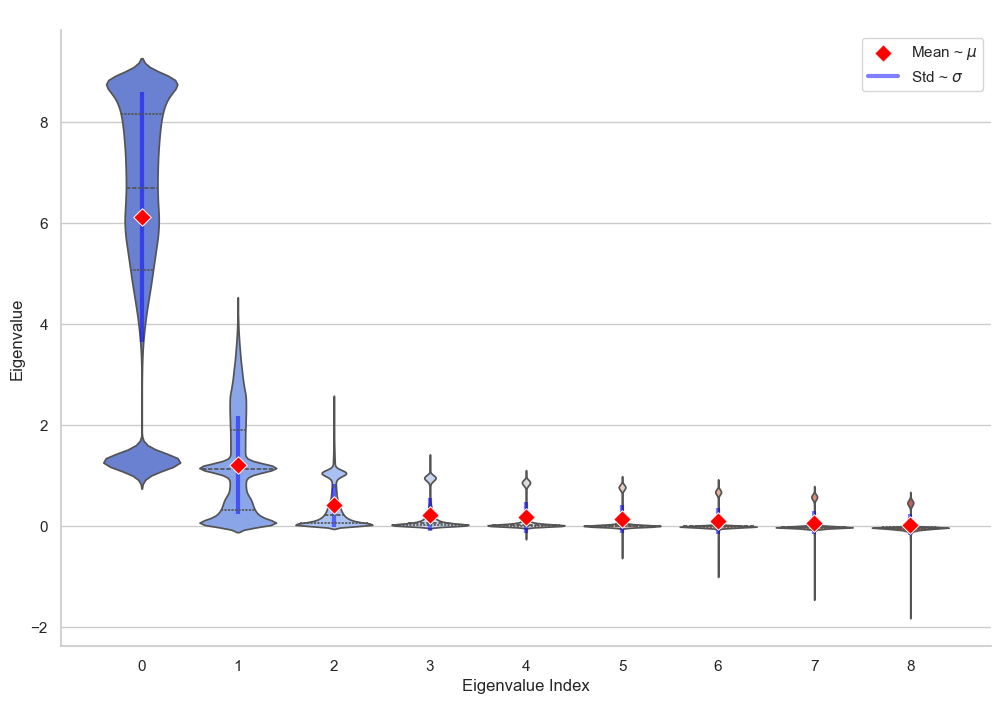
\includegraphics[width=0.5\textwidth]{figures/06_ModelExploration/1_InputData/eigval_violin_raw.png}}}
    \subfloat[]{{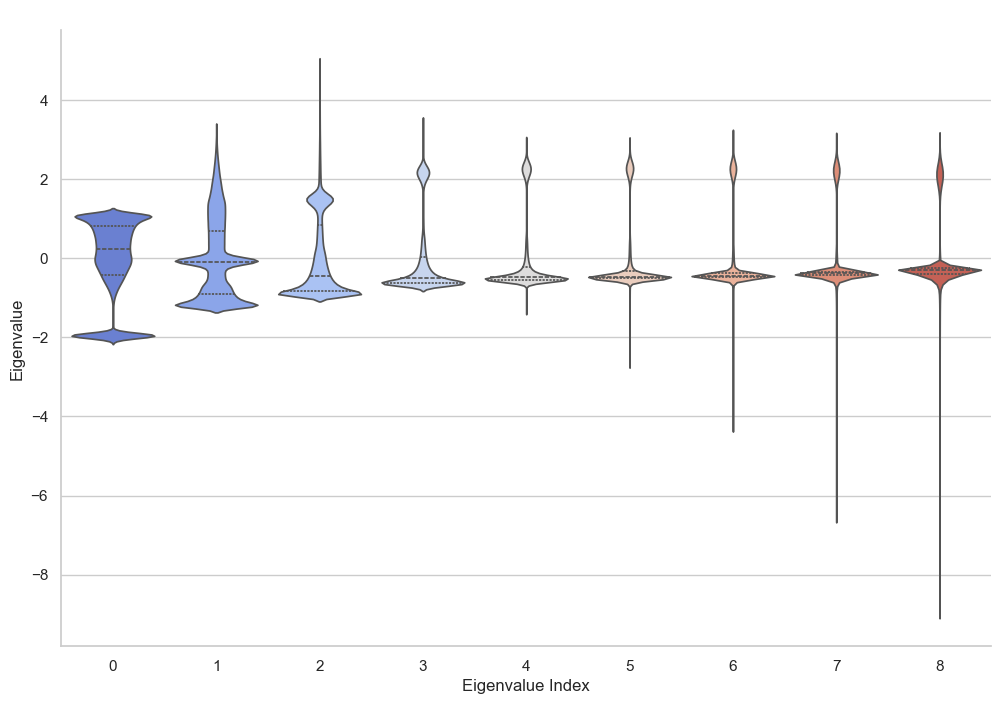
\includegraphics[width=0.5\textwidth]{figures/06_ModelExploration/1_InputData/eigval_violin_norm.png}}}
    \caption{Distributions of the eigenvalues \( \bfL \) before (a) and after (b) index-wise normalization.}
    \label{fig:eigenvalues_norm}
\end{figure}

The violin plot of the unnormalized
eigenvalues, shows that the eigenvalues, belonging noise-only scenarios, are clustered around the noise variance \( \sigma^2_{\eta} = 1\si{\micro\volt\squared}\),
and that an intuitive manual separation of the signal and noise eigenvalues is in most cases only possible for \( N < 3 \).
\hyperref[fig:eigenvalues_norm]{Figure~\ref*{fig:eigenvalues_norm}a} also depicts the mean and standard deviation of the
unnormalized eigenvalues, which additionally are gathered in \autoref{tab:dataset_stats}.

\begin{table}[H]
    \centering
    \caption{Statistics of Training Dataset Eigenvalues}
    \label{tab:dataset_stats}
    \begin{tabular}{lrrrrrrrrr}
    \toprule
    & \multicolumn{9}{c}{\textbf{Eigenvalue Index}} \\
    \cmidrule{2-10}
    & 1 & 2 & 3 & 4 & 5 & 6 & 7 & 8 & 9 \\
    \midrule
    \( \mu_i \) & 6.122 & 1.220 & 0.419 & 0.236 & 0.179 & 0.143 & 0.110 & 0.075 & 0.035 \\
    \( \sigma_i \) & 2.478 & 0.973 & 0.428 & 0.334 & 0.305 & 0.279 & 0.253 & 0.229 & 0.203 \\
    \bottomrule
    \end{tabular}
\end{table}



The evaluation of index-wise normalization's role in enhancing the predictive capabilities of an early \gls{cnn} iteration,
is detailed in \autoref{tab:model_performance}.

\begin{table}[H]
    \centering
    \caption{Impact of input data normalization on model performance}
    \label{tab:model_performance}
    \begin{tabular}{@{}lcccccc@{}}
    \toprule
    & \multicolumn{2}{c}{\( \meanLossCEVal \)} & \multicolumn{2}{c}{ \( \meanAccVal \)} & \multicolumn{2}{c}{\#MACs} \\
    \cmidrule(lr){2-3} \cmidrule(lr){4-5} \cmidrule(lr){6-7}
    Normalization & \( \nu \) & \( \%\Delta \) & \( \nu \) & \( \%\Delta \) &  &\\
    \midrule
    False & 0.616 & — & 0.725 & — &  — \\
    True & 0.615 & \gnbx{-0.30\%} & 0.726 & \gnbx{0.06\%} & \redbigoplus{} \\
    \bottomrule
    \end{tabular}
\end{table}

The results in \autoref{tab:model_performance} indicate that the index-wise normalization yields only a marginal improvement in the
model's performance, with a slight decrease in the mean validation loss%
\footnote{
    \( \meanLossVal \coloneq \mathbb{E}_{(\mbf{Z}, \mbf{Y}_N) \sim \DVal}[\lossCEVal(\mbf{Z}, \dot{\mbf{Y}}_N)]\), \( \mbf{Z} \) being
    the model's logits, and \( \dot{\mbf{Y}}_N \) the one-hot encoded ground truth labels.
}.
and a neglectable increase in the validation accuracy,
while coming at the cost of an increased number of \glspl{mac} through the additional normalization operations.


\subsubsection{Reevaluation of Index-wise Normalization}
\label{subsubsec:reevaluation_index_wise_normalization}

Upon retrospective reflection of the index-wise normalization approach, several insights have emerged that warrant
reconsideration of its appropriateness for the task at hand.

Firstly, the examination of the eigenvalue distribution underscores a relatively constrained variance, particularly
highlighted by a manageable peak to peak spread and level difference:
\begin{align*}
    \Delta\lambda_{pp} &= \max(\bfLT^{\D}_{:,:}) - \min(\bfLT^{\D}_{:,:}) \approx 11.2\si{\micro\volt\squared}, \\
    L_{\mu,pp} &= L_{\mu_1} - L_{\mu_M} = \num{44.9}\si{\decibel}.
\end{align*}

The practice of index-wise normalization, while theoretically enhancing uniformity across eigenvalue magnitudes,
amplifies the variability of lower-magnitude eigenvalues due to their low relatively low standard deviation and the
resulting inherent reciprocal scaling effect on outliers. This increased spread would mostly affect noise eigenvalues,
whose values might not encode any meaningful information about the model order, due to the effects of sub-sampling.
Enforcing uniformity across the priorities of all eigenvalues might not be aligned with the task's inherent
requirements.

Another argument advocating against normalization is the fact that the mean and standard deviation of some eigenvalues
exhibit low absolute values, which would exacerbate numerical errors in low-precision computational environments.
The subtraction of two relatively small numbers and the subsequent division by a small number would most likely lead to
the occurrence of high numerical errors, especially in the case of hardware implementation, which would require lower
precision fixed-point numbers.

Given the neglectable performance gain and the additional computational cost, the low complexity of the input data, and
the aforementioned detrimental effects, it was decided not to utilize the normalized eigenvalues as input data for the
networks.



% \section{Previous Deep Learning Approaches}
% [\cite{yang2020}]
% ```
% Based on information theory [6], the covariance matrix C contains the key information for the source number detection. One natural idea is to employ DNN to learn the source number directly from the covariance matrix C. However, it is would not be an effective way to to so due to the information redun- dancy in C that contains all unknown information besides the number of sources (will be verified in simulations).
% Although DL exhibits powerful learning capability in extracting features from massive data, model information, if can be well utilized, would provide significant enhancement in performance [11]. To see this, let us express C as

% where lambda and um are the m-th eigenvalue and correspond- ing eigenvector of C, respectively. From the array signal processing theory [5], the eigenvectors would construct the signal subspace and the noise subspace, from which the ESPRIT and MUSIC algorithms can be applied to estimate the DOA, respectively. Nevertheless, it is clearly that eigenvectors themselves do not contain information of the number of the sources and hence would bring redundancy if being input to the DNN. Hence, instead of input the whole C, we propose to only input the DNN the eigenvalues , which is also consistent with the AIC and MDL approaches. Notice that the eigenvalues  are all real numbers, therefore, complex operations are not required in the proposed ERNet and ECNet.
% ```
% They employed a fully connected NN, and no sub-sampling
% + Eigenvalues and Eigenvectors are \( \in \mathbb{R} \) and not complex such as the covariance matrix
% + \cite{yang2020} showed <überlegene> performance of eigenvalues over covariance matrix in for non-coherent sources and varying numbers of snapshots
% - \cite{yang2020} When the sources are coherent, which is the common in the real environment, the signal covariance matrix is rank- deficient, and therefore the performance of eigenvalue based methods degrades [16]. To solve the problem, the FBSS scheme is adopted [9], where the the total array of M antennas is divided forward/backward into overlapping sub-arrays with size M 0. The number of forward/backward sub-arrays is T = M - M0 + 1. Note that the M0 >     K and T >= K should be satisfied as proved in [16]. Then, the forward/backward averaged covariance matrix is given by [9]


\section{Choice of Optimization Objective}

\subsection{Regression}
When faced with the challenge of estimating discrete ordinal quantities, such as the number of sources in model order estimation tasks,
the initial inclination might lean towards employing regression models.
At first glance, these models offer a straightforward approach, potentially allowing for the interpretation of their
quasi-continuous output as a discrete source count after appropriate rounding.\\
However, this method exhibits intrinsic limitations due to the absence of inherent output bounds in regression models,
leading to the necessity for artificial scaling interventions.

Solutions like applying a scaled sigmoid function to the regression layer's output have been contemplated to confine the
predictions within the required range of \( [0, N_{\max}] \).\\
Despite its theoretical viability, this approach inadvertently biases the model towards mid-range values,
complicating the differentiation between adjacent classes, especially at the boundary values.

A more feasible alternative is to transform the output of the regression layer according, would be to round it to
the nearest integer and clamp it, such that it falls within the valid range of source counts.
% Add a brief explanation of ˜\hat{bfm{y}}_reg˜ - single neuron output -> #Params in regression layer: # CHs_prev_layer * 1
\begin{equation}
    \bfm{\NPred}_{\text{reg}} = \max\left(0,\:\min(N_{\max},\:\nint{\hat{\bfm{y}}})\right), \quad \hat{\bfm{y}} \in \mathbb{R}^{\B}, \: \bfm{\NPred}_{\text{reg}} \in \NSet^{\B}
    \label{eq:regression_clamp}
\end{equation}

Similarly to~\cite{yang2020} we decided to employ the \gls{mse} (\( \mathcal{L}_2 \)) loss function for the regression model.
\begin{equation}
    \lossMSE(\hat{\bfm{y}}, \bfm{N}) = \frac{1}{\B} \sum_{i=1}^{\B} \left(\hat{y}_i - N_i\right)^2, \quad \hat{y}_i \in \mathbb{R},\: N_i \in \NSet
    \label{eq:mse_loss}
\end{equation}

\subsection{Classification}
For convenience, let \( C \coloneq N_{\max} + 1 = \| \NSet \| \) denote the number of classes in the classification task.\\
The classification approach provides a more intuitive and efficient solution to the task. Rather than using a regression
layer with a single neuron output, we utilize a classification layer that produces a tensor of logits \( \bfm{Z} \in \mathbb{R}^{\B \times C}\).
This enables the classification model to have separate output units for each class.\\
To denote the logits vector for a specific sample within the batch, let \( \bfm{z} \coloneq \bfm{Z}_{b,:} \),
where \( \bfm{z} \in \mathbb{R}^{C} \) represents the logits for the \( b \)-th sample across all \( C \) classes.\\
The interpretation of each element within the logits vector \( \bfm{z} \) corresponds to the log-likelihood for class
memberships, where \( z_c = \ln \Pr(N=c|\bfL; \bfm{\omega}) \) represents the logarithm of the probability that
the model order \( N \) equals class \( c \), conditioned on the input \( \bfL \) and parameterized by the model weights
\( \bfm{\omega} \)~\cite[Chapter 6]{dlbook}.

During inference, the model order estimate \( \NPred_{\text{cls}} \) is obtained by determining the index of the maximum element in
the logits vector \( \bfm{z} \):
\begin{equation}
    \bfm{\NPred}_{\text{cls}} = \argmax_{c \in \NSet} \bfm{Z}_{:,c}, \quad \bfm{\NPred}_{\text{cls}} \in \NSet^{\B}
    \label{eq:classification_argmax}
\end{equation}

For the purpose of training, however, the softmax activation function is applied to the logits, converting them into a valid probability
distribution across the class labels. The transformation \( \mathrm{softmax} : \mathbb{R}^C \rightarrow [0, 1)^C \) is defined by:
\begin{equation}
    \hat{y}_c = \text{softmax}(\bfm{z})_c = \frac{e^{z_c}}{\sum_{j=1}^{C} e^{z_j}}, \quad c \in \NSet
    \label{eq:softmax}
\end{equation}
where \(\hat{y}_c\) represents the predicted probability that the model assigns to class \(c\), given the logits
vector \(\bfm{z}\) for a specific sample. The softmax function ensures that the output probabilities sum to one,
facilitating a direct comparison with the true class labels.

Consequently, the cross-entropy loss function is utilized to quantify the discrepancy between the predicted probability
distribution and the true label distribution and is defined as follows:
\begin{equation}
    \lossCE(\hat{\bfm{Y}}, \dot{\mbf{Y}}_N) = -\frac{1}{\B} \sum_{b=1}^{\B} \sum_{j=1}^{C} N_{bj} \ln(\hat{y}_{bj}), \quad \dot{\mbf{Y}}_N, \hat{\bfm{Y}} \in \mathbb{R}^{\B \times C}
    \label{eq:ce_loss}
\end{equation}
In \autoref{eq:ce_loss}, \( \dot{\mbf{Y}}_N \) represents the true class labels in one-hot encoding. Each row of \( \hat{\bfm{Y}} \),
denoted as \( \hat{\bfm{y}} = [\hat{y}_1, \ldots, \hat{y}_c] \), represents the model's predicted probabilities for a particular sample.

\subsection{Comparison and Conclusion}

\begin{figure}[H]
    \centering
    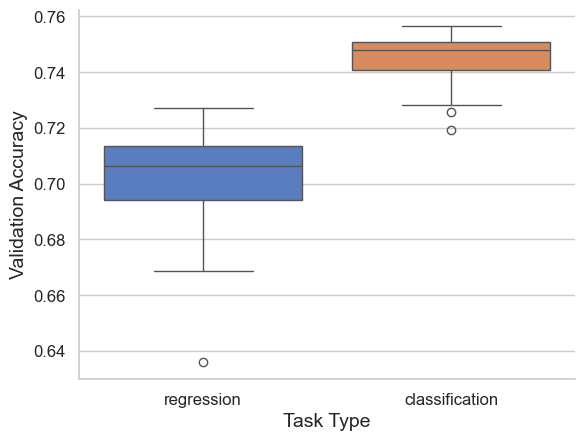
\includegraphics[width=0.45\textwidth]{figures/06_ModelExploration/conv_task_type.png}
    \caption{Boxplot of \( \meanAccVal \) for the regression and classification tasks.}
    \label{fig:task_type}
\end{figure}

Figure~\ref{fig:task_type} compellingly demonstrates the superior performance of the classification paradigm over
regression in terms of validation accuracy. A brief explanation of the employed boxplots is provided in~\autoref{app:sec:Boxplot}.
To quantify this advantage,~\autoref{tab:accuracy_change} details the relative improvement when switching from regression
to classification.

\begin{table}[H]
    \centering
    \caption{Quantitative Performance Metrics: Regression vs. Classification}
    \label{tab:accuracy_change}
    \begin{tabular}{@{}lcc@{}}
    \toprule
    & \multicolumn{2}{c}{\( \meanAccVal \)} \\
    \cmidrule(lr){2-3}
    Task Type & \( \nu \) & \( \%\Delta \) \\
    \midrule
    Regression~\bigoplus~\( \lossMSE \) & 0.7062 & — \\
    Classification~\bigoplus~\( \lossCE \) & 0.7478 & \gnbx{+5.889\%} \\
    \bottomrule
    \end{tabular}
\end{table}

The data presented in \autoref{tab:accuracy_change} as well as the boxplots in \autoref{fig:task_type} were obtained by optimizing for
the respective loss functions \( \lossMSE \) and \( \lossCE \) on the validation set \( \DMain_{(\text{val})} \) using an
earlier the \gls{cnn} architecture, which will be introduced in \autoref{sec:cnn}.


The only downside of employing the classification approach is an increase in computational cost due to the
additional \( C - 1 \) neurons in the output layer. Assuming a total of \( K_{\text{CH}} \) channels or features in the
previous layer, the number of parameters in the output layer for both tasks given by:
\begin{align}
    \#\text{Params}_{\text{head,reg}} &= K_{\text{CH}} \times 1 \\
    \#\text{Params}_{\text{head,cls}} &= K_{\text{CH}} \times C
\end{align}

This increased computational cost is a small price to pay for the significant improvement in performance, which is
why we decided to proceed with the classification approach for the remainder of the study. Both, the softmax activation
function and the multi-class cross-entropy loss function are embedded into the categorical cross-entropy loss function
that is provided by the \textsc{PyTorch} library.

Given the applicability of cost functions like \gls{mse} \( \loss^{\text{MSE}} \) regardless of the task type, it might
be worthwhile to explore the use of \gls{mse} or a similar loss function with an emphasis on the regressive nature of
the output, in a hybrid approach in combination with the softmax \( \oplus \) cross-entropy loss.

\section{Convolutional Neural Network}
\label{sec:cnn}
\subsection{Hyperparameter Optimization}

\subsubsection{Convolutional Layers}

Convolutional layers are the core of the \gls{cnn} architecture by harnessing three key concepts—sparse interactions,
parameter sharing, and spatially equivariant feature representations—that collectively contribute to a robust and efficient
component for feature extraction~\cite[Chapter 9]{dlbook}. \\
These layers employ multiple kernels (\( \coloneqq \) filters) that extend across all channels of the input data and perform
a convolution through the spatial dimension of the input sequence. \\
Our input data to the one-dimensional convolutional layers (\texttt{nn.Conv1d}) can be perceived as a
sequence of eigenvalues with length \(  L_{\text{seq}} = M \), exhibiting a single channel \( C_{\text{in}} = 1\), or
as a singleton sequence with \( C_{\text{in}} = M \) channels. \\
Each filter produces a feature map, representing the presence of specific patterns detected in the input, with the number
of output channels in a convolutional layer corresponding to the number of these finite impulse response filters.

\textbf{The Number of Channels} presents a critical hyperparameter that dominates the model's capacity for feature detection.

\begin{figure}[H]
    \centering
    \subfloat[]{{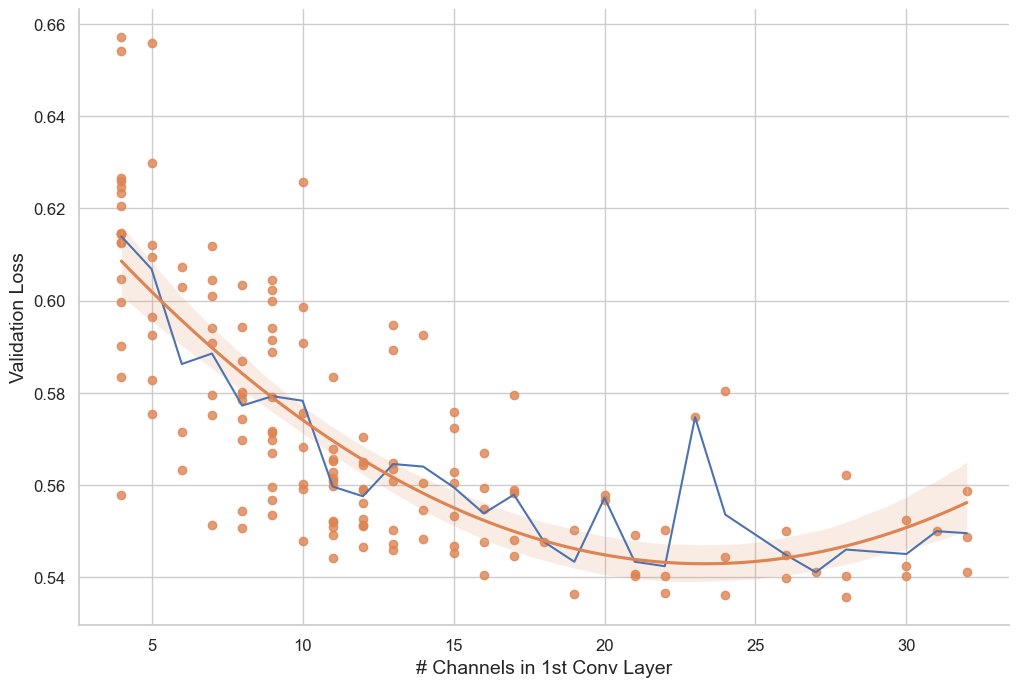
\includegraphics[width=0.48\textwidth]{figures/06_ModelExploration/4_CNN/conv_ch1.png}}}
    \subfloat[]{{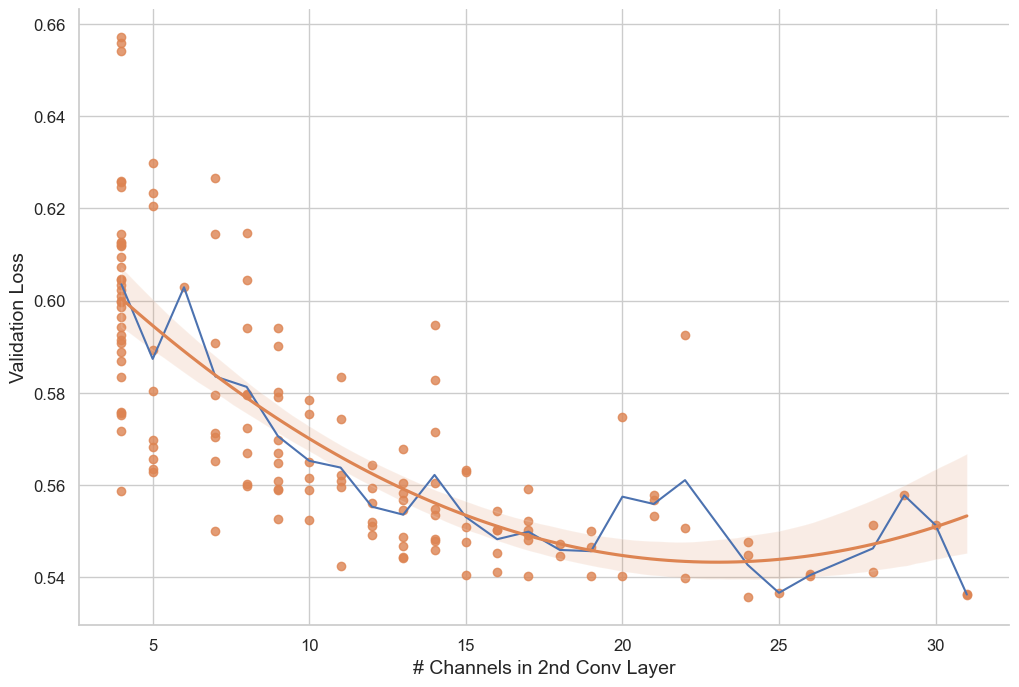
\includegraphics[width=0.48\textwidth]{figures/06_ModelExploration/4_CNN/conv_ch2.png}}}
    \caption{Influence of the number of channels in the first (a) and second (b) convolutional layers on \( \lossCEVal \).}
    \label{fig:ch1ch2}
\end{figure}

\begin{figure}[H]
    \centering
    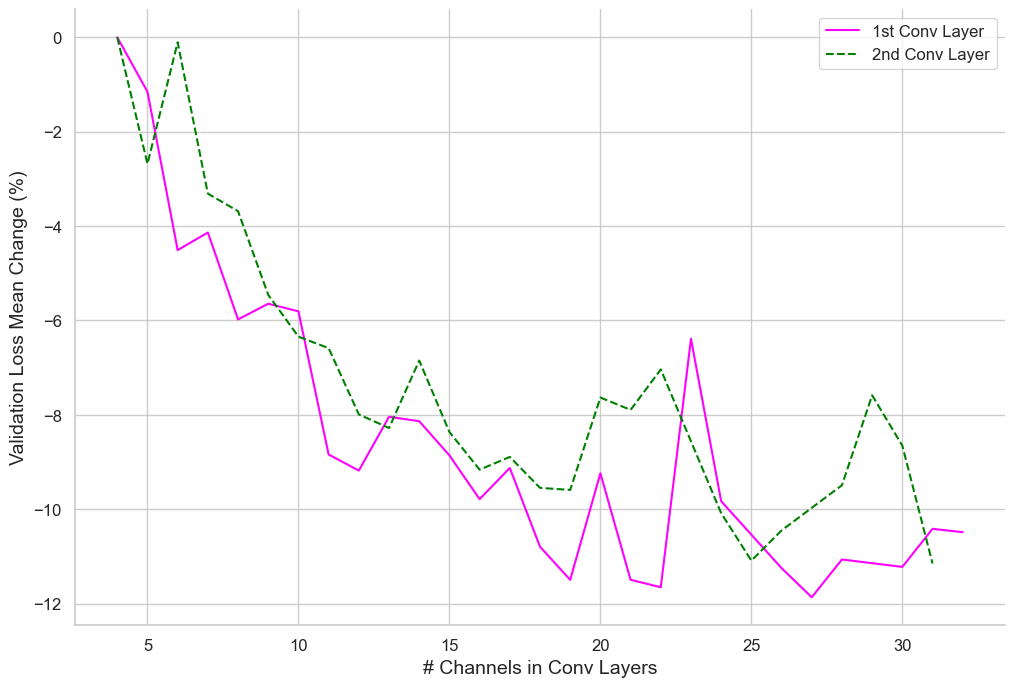
\includegraphics[width=0.5\textwidth]{figures/06_ModelExploration/4_CNN/conv_ch_change.png}
    \caption{Relative changes in validation loss for varying number of channels in both conv blocks.}
    \label{fig:ch1ch2_relchange}
\end{figure}

Figures~\ref{fig:ch1ch2} and~\ref{fig:ch1ch2_relchange} illustrate how varying the number of channels affects model
performance, guiding the selection towards an optimal balance that maximizes feature extraction while minimizing the
likelihood of overfitting.\\
Both figures indicate that the explored ranges of channels \( C_{\text{out}} \) were chosen appropriately, given that
the validation loss \( \lossCEVal \) exibits a local minimum, beyond which the loss increases due to overfitting. \\

\textbf{Pooling Layers} complement convolutional layers by reducing the spatial dimension of the feature maps,
thus allowing the model to capture higher-level features with a greater local dispersion. \\

The sizes of the pooling windows as well as other hyperparameters which are linked to the convolutional layers, all have
an impact on the model's performance, as depicted in Figure~\ref{fig:param_impact}.

\begin{figure}[H]
    \centering
    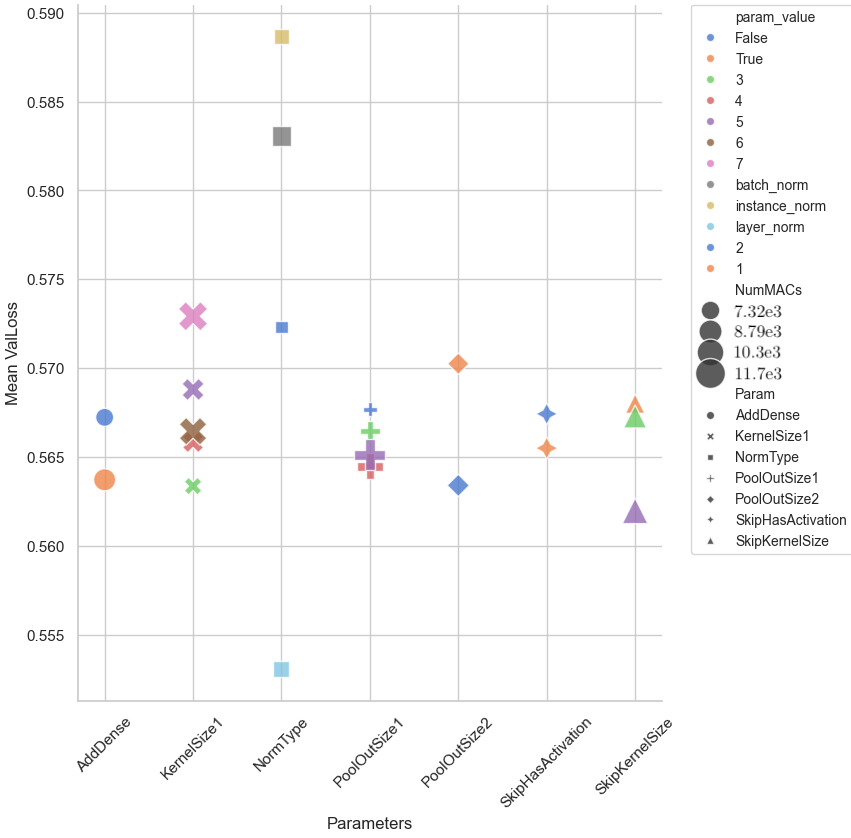
\includegraphics[width=0.6\textwidth]{figures/06_ModelExploration/4_CNN/scatter.png}
    \caption{Scatter plot showing the impact of different hyperparameters on mean validation loss.}
    \label{fig:param_impact}
\end{figure}

Figure~\ref{fig:param_impact} presents a scatter plot of various hyperparameter configurations and their corresponding
mean validation loss. Each point represents a unique combination of parameters such as kernel size, normalization type,
and pooling size. The plot indicates the sensitivities of the validation loss to these hyperparameters, with certain
configurations leading to lower loss values and thus better model performance.

The scatter plot also highlights the trade-offs between model complexity, as indicated by the size of the points
representing the number of \glspl{mac}.\\
For example, larger kernels and additional dense layers may contribute
to a lower validation loss but also increase the computational requirements. Conversely, smaller kernels and fewer dense
layers might yield a less complex model but potentially at the cost of higher validation loss.

The other depicted criteria, such as the type of normalization layer, will be discussed subsequently.

\subsubsection{Normalization Layers}
Normalization layers, crucial for modern deep networks, standardize the activations of each layer,
thus enhancing the optimization process and the network's generalization capabilities. \\
Even in shallow networks, normalization proves beneficial, as it stabilizes the gradient flow by reducing the sharpness
of the loss surface. \\
A smoother loss surface is associated with a reduced risk of overfitting since it is less likely
to contain sharp local minima, which are more prone to overfitting and generally hinder the optimization process~\cite{lyu2023norm}.\\
Another advantage is the reduction of the internal covariate shift, which is the change in the distribution of network's activations during training, as
well as the consequent potential for faster convergence through the employment of larger learning rates. \\

In the context of this work, three normalization layers were considered: Batch Normalization, Instance Normalization,
and Layer Normalization, each visualized in~\autoref{fig:all_norm_types}.

\begin{figure}[H]
    \centering
    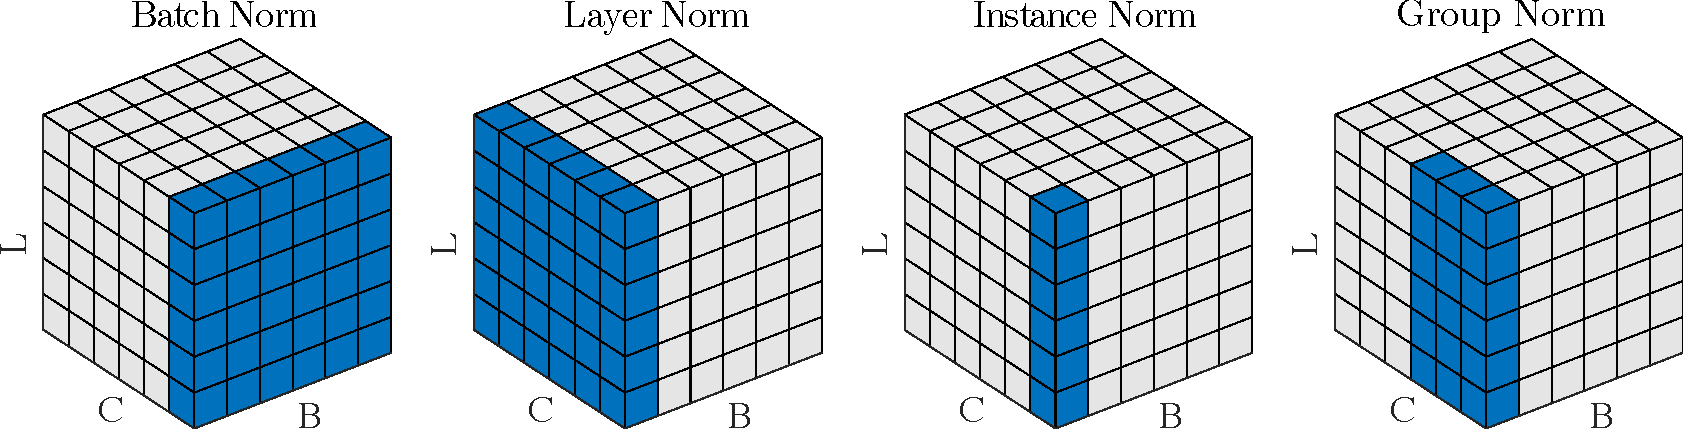
\includegraphics[width=0.6\textwidth]{figures/06_ModelExploration/4_CNN/all_norms.pdf}
    \caption{Feature map tensors -- blue units are normalized by the same mean and variance~\cite{wu2018group}.}
    \label{fig:all_norm_types}
\end{figure}

Although, Group Normalization was not considered in this work, it is worth mentioning it, since it was shown to outperform
the other normalization layers in the context of small batch sizes~\cite{wu2018group}, while being on par with Group Norm for larger batch
sizes, while exhibiting no dependence on the batch size. \\
Batch Normalization computes statistics (\(\mathbb{E}[\bfm{X}], \operatorname{Var}[\bfm{X}]\)) across the spatial
dimensions and all samples in the mini-batch for each channel, Layer Normalization along the \((L, C)\) axes for each
sample, and Instance Normalization along the \(L\) axis for each sample and channel~\cite{wu2018group}.

They all aim to compensate for the possible loss of representational capacity by introducing a learnable linear
transformation, parametrized by \( \bfm{\gamma} \) and \( \bfm{\beta} \),
that scales and shifts the normalized value~\cite{wu2018group}, expressed for Layer Normalization as~\cite{PyTorchLayerNorm}:
\begin{equation}
    \bfm{Y}_{b, :, :} = \bfm{\gamma} \odot \left( \frac{\bfm{X}_{b, :, :} - \mathrm{E}[\bfm{X}_{b, :, :}]}{\sqrt{\operatorname{Var}[\bfm{X}_{b, :, :}] + \epsilon}} \right) + \bfm{\beta}, \quad \text { where } \bfm{\gamma}, \bfm{\beta} \in \mathbb{R}^{C \times L}
\end{equation}

The validation loss for each normalization layer is depicted in~\autoref{fig:norm_type}.
\begin{figure}[H]
    \centering
    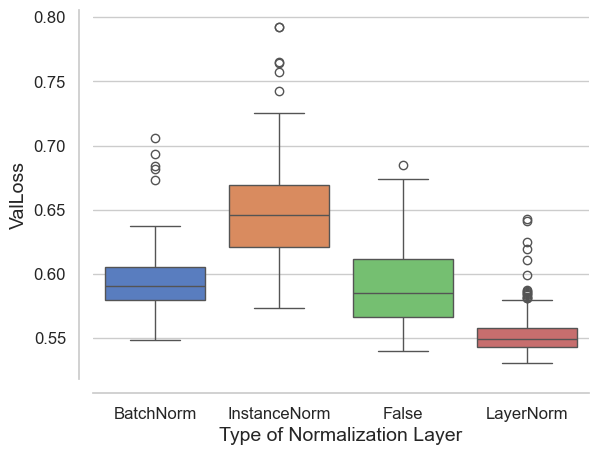
\includegraphics[width=0.6\textwidth]{figures/06_ModelExploration/4_CNN/conv_norm_type.png}
    \caption{Validation loss for different normalization layers.}
    \label{fig:norm_type}
\end{figure}

As shown in~\autoref{fig:norm_type}, the application of layer normalization (Layer Norm) resulted in the lowest \( \meanLossCEVal \),
while Instance Norm and Batch Norm performed worse. The respective layer's impacts on the model's performance and complexity
are summarized in~\autoref{tab:norm_type}.

\begin{table}[H]
    \centering
    \caption{Comparison of different normalization layers and their effects on mean validation loss and model complexity.}
    \label{tab:norm_type}
    \begin{tabular}{@{}lcccccccc@{}}
    \toprule
    & \multicolumn{2}{c}{\( \meanLossCEVal \) } & \multicolumn{2}{c}{\( \meanAccVal \)} & \multicolumn{2}{c}{\#Params} & \multicolumn{2}{c}{\#MACs} \\
    \cmidrule(lr){2-3} \cmidrule(lr){4-5} \cmidrule(lr){6-7} \cmidrule(lr){8-9}
    Normalization & \( \nu \) & \( \%\Delta \) & \( \nu \) & \( \%\Delta \) & \( \nu \) & \( \%\Delta \) & \( \nu \) & \( \%\Delta \) \\
    \midrule
    None               & 0.590 & —            & 0.737 & —            & 2322 & —    & 7.01e3 & — \\
    Batch Norm          & 0.596 & \rdbx{+0.98\%} & 0.732 & \rdbx{-0.573\%} & 2787 & \rdbx{+20.0\%} & 10.7e3 & \rdbx{+53.6\%} \\
    Instance Norm       & 0.648 & \rdbx{+9.91\%} & 0.712 & \rdbx{-3.31\%}  & 2858 & \rdbx{+23.1\%} & 10.6e3 & \rdbx{+52.3\%} \\
    Layer Norm          & 0.553 & \gnbx{-6.16\%} & 0.748 & \gnbx{+1.61\%}  & 3414 & \rdbx{+47.0\%} & 9.52e3 & \rdbx{+35.8\%} \\
    \bottomrule
    \end{tabular}
\end{table}


The underwheling performance of Instance Norm is likely due its inherent unsuitablity for the task at hand, given that
it was originally designed for style transfer and image generation tasks and generally requires larger spatial or temporal
dimensions to effectively estimate the mean and variance of the input data.
Moreover, Instance Norm was \emph{not} implemented with the subsequent affine transformation, which also contributed to its
underperformance.\\
Layer Norm has demonstrated its capability to address various shortcomings of Batch Norm~\cite{ba2016layer}, although
such shortcomings were not expected to be significant in this context.

Surprisingly, Batch Norm's performance was not as strong as anticipated, despite its common application in \gls{cnn} architectures
and the use of a relatively large batch size \( \B = 1024 \). The most likely explanation is that the optimization process
was conducted with a dropout rate of eight percent in each convolutional block.
Since both Batch Norm and Dropout layers introduce noise to the optimization process, their combined use could have
hindered optimal convergence. \\
It would be worthwhile to investigate Batch Norm's performance without the inclusion of dropout layers, as it is
hypothesized to surpass Layer Norm's performance when considering the large batch size~\cite{wu2018group}.


Layer Norm distinguished itself among the normalization techniques evaluated, offering superior model performance and lower complexity. \\
The advantage of Layer Norm over Batch Norm, in terms of the number of \glspl{mac}, seems paradoxical.
Batch Norm separates the entire mini-batch into \( C \) independent normalization groups, whereas Layer Norm normalizes
each sample independently. Considering that \( \B \gg C \), and \( \text{\#Params}_{\text{LN}} = L \cdot \text{\#Params}_{\text{BN}} \),
this result appears counterintuitive. \\



\subsubsection{Activation Function}
Activation functions play a critical role in neural networks, introducing non-linear properties to the system,
which allows the model to learn complex non-linear patterns in the data. The choice of activation function can
significantly affect the learning dynamics and performance of the network.

Traditionally, the \gls{relu} has been widely used due to its simplicity, effectiveness in addressing the vanishing
gradient problem, and its advantageous effects on the convergence of the optimization process over activation functions that
introduce non-zero second derivatives~\cite[Chapter 6.3.1]{dlbook}.\\
However, \gls{relu} can introduce ``dead units'', which are neurons that never activate, and therefore bring no contribution
to the network's discriminative and predictive capabilities.\\
To overcome this, variations like leaky \gls{relu}, \gls{prelu} and \gls{elu} have been proposed, which allow a small,
positive gradient for negative input values, thus preventing the issue of dead units and allowing higher learning rates~\cite{dyingRelu}.

The equations defining each activation function are as follows:

\begin{align}
    \texttt{ReLU}(x) &= \max(0, x) \label{eq:relu} \\
    \texttt{PReLU}(x) &= \begin{cases}
        x & \text{if } x > 0 \\
        \alpha x & \text{if } x \leq 0
    \end{cases}, \quad \text{where } \alpha \text{ is a learnable parameter} \label{eq:prelu} \\
    \texttt{ELU}(x) &= \begin{cases}
        x & \text{if } x > 0 \\
        \alpha \left( e^x - 1 \right) & \text{if } x \leq 0
    \end{cases}, \quad \text{where } \alpha = 1 \text{ per default}\label{eq:elu}
\end{align}

\begin{figure}[H]
    \centering
    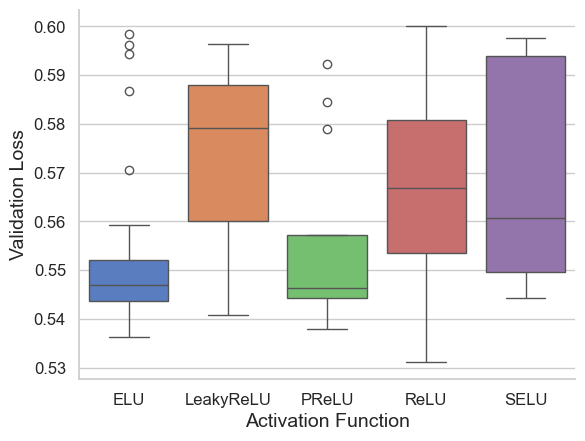
\includegraphics[width=0.55\textwidth]{figures/06_ModelExploration/4_CNN/activ_fn.png}
    \caption{Boxplots of \( \lossCEVal \) for different activation functions.}
    \label{fig:activ_fn}
\end{figure}

\autoref{fig:activ_fn} demonstrates the influence of activation functions on model performance through the distribution
of validation loss. Among the evaluated functions, \gls{prelu} and \gls{elu} show a slight advantage over \gls{relu} in terms of validation
loss, indicating potential improvements in learning dynamics and model robustness. \\
The advantages of \gls{prelu} and \gls{elu} over \gls{relu} are further quantified in \autoref{tab:activation_fn}.

\begin{table}[H]
    \centering
    \caption{Comparison of Validation Loss for Different Activation Functions}
    \label{tab:activation_fn}
    \begin{tabular}{@{}lcc@{}}
    \toprule
    Activation Function & \multicolumn{2}{c}{\( \meanLossCEVal \) } \\
    \cmidrule(lr){2-3}
                      & \( \nu \) & \( \%\Delta \) \\
    \midrule
    \gls{relu}    & 0.567 & —           \\
    \gls{prelu}   & 0.555 & \gnbx{-2.10} \\
    \gls{elu}     & 0.551 & \gnbx{-2.69} \\
    \bottomrule
    \end{tabular}
\end{table}

\gls{elu}'s smoother transition from negative to positive inputs theoretically benefits learning dynamics but
comes at a higher computational cost due to the exponential function, which might be disadvantageous for deployment on resource-constrained platforms like \glspl{fpga}.
Conversely, \gls{prelu} offers a compromise by introducing a learnable parameter, \( \alpha \), that adjusts the slope for negative inputs, offering flexibility without
significantly increasing computational demands. For this reason, \gls{prelu}, with a single shared \(\alpha\) parameter across
channels, is chosen for its balance between performance improvement and computational efficiency.
This consideration ensures that the selected activation function optimizes learning while remaining feasible for deployment
on resource-constrained platforms.

\subsubsection{The Resulting CNNP Block}
\label{subsubsec:cnn_block}

The construction of the \texttt{CNNP} block represents a synthesis of empirical findings from the exploratory process
and theoretical considerations, yielding a composite layer structure within the convolutional neural network framework.

It comprises a sequential arrangement of a one-dimensional convolutional layer (\texttt{nn.Conv1d}), followed by a
layer normalization module (\texttt{nn.LayerNorm}), a parametric rectified linear unit (\texttt{nn.PReLU}), and an
adaptive max pooling layer (\texttt{nn.AdaptiveMaxPool1d}), concluding with a dropout layer to mitigate overfitting.

\[
    \texttt{CNNP} \coloneqq \underbrace{\texttt{nn.Conv1d}}_{\text{\textbf{C}onv}}
    \rightarrow \underbrace{\texttt{nn.Layer Norm}}_{\text{\textbf{N}orm}}
    \rightarrow \underbrace{\texttt{nn.PReLU}}_{\text{\textbf{N}on-linear}}
    \rightarrow \underbrace{\texttt{nn.AdaptiveMaxPool1d}}_{\text{\textbf{P}ool}}
    \rightarrow \texttt{nn.Dropout}
\]

The dropout rate was optimized parallel to the other hyperparameters, depicted in~\autoref{fig:param_impact}, and its
impact on the model's performance can be found in the appendix~\autoref{fig:dropout_cnn}.


\subsubsection{Skip Connection}

Skip connections, are a fundamental architectural feature in deep neural networks that enable the training of significantly
deeper models by providing advantageous optimization trajectories through the loss landscape or allowing for the reuse or
preservation of important features throughout the network. \\
The most prominent example of a skip connection is the residual connection, which was first introduced in the ResNet architecture~\cite{he2015deep}.
Residual connections aim to address the degradation problem, which is the phenomenon where increasing the depth of a network
results in higher training error due to various optimization difficulties. \\
The application of residual connections mostly aims to achieve better optimization dynamics by reformulating the
bypassed layers' training objectives to learn the residual (\( \coloneq \) difference) from the identity mapping, instead
of learning an unreferenced mapping from scratch.

Since the phenomenon of degradation is more prevalent in very deep networks, which might be up to 2 orders of magnitude deeper
than our model, the use of skip connections is not motivated by the degradation problem, but rather by the goal to allow
for more diverse feature representations.
The use of skip connections in our model architecture is motivated by the
desire to create an ensemble of the two parallel paths, which can be seen as an ensemble of the serially connected
\texttt(CNNP)s and a layer that performs the operation formalized in~\autoref{eq:skip_connection}.
\begin{equation}
    \bfm{X}_{:, j}^{\text{(skip)}} = \texttt{ReLU}\left(\text{bias}_j + \sum_{k=0}^{M} \bfLT_{:, k, 1}^P \cdot W_{jk}\right), \quad  \bfm{X}^{\text{(skip)}} \in \mathbb{R}^{\B \times C_{\text{out}}^{(\text{skip})}}, \: j = 1, \ldots, C_{\text{out}}^{(\text{skip})}
    \label{eq:skip_connection}
\end{equation}
The input to the skip connection is the permuted tensor of eigenvalues \( \bfLT^P \coloneqq \texttt{permute}( \bfLT, [0, 2, 1] ) \).
\( C_{\text{in}}^{(\text{skip})} = M = \| \bfL \| \) is the number of input channels, \( C_{\text{out}}^{(\text{skip})} \)
is the number of output channels, and \( \bfm{W} \) are the weights of the \( 1 \times 1 \) convolutional layer in the
skip connection.

In contrast to a residual connection, the outputs of our skip connection \( \bfm{X}^{\text{(skip)}} \) are not
added to the outputs of the ``main'' path, but are concatenated to them. \\
Adding the outputs of the skip connection and the main path requires both operands to exhibit the same dimensions, which is
not the case in our model architecture. Moreover, concatenation preserves a more diverse feature representation since
it allows both paths to learn different features, rather than simplifying the learning task by allowing the model to
learn the residual from the identity mapping. \\

\begin{table}[H]
    \centering
    \caption{Comparison of model performance with and without skip connections}
    \label{tab:residual_comparison}
    \begin{tabular}{@{}lcccccccc@{}}
    \toprule
    & \multicolumn{2}{c}{\( \meanLossCEVal \) } & \multicolumn{2}{c}{\( \meanAccVal \)} & \multicolumn{2}{c}{\#Params} & \multicolumn{2}{c}{\#MACs} \\
    \cmidrule(lr){2-3} \cmidrule(lr){4-5} \cmidrule(lr){6-7} \cmidrule(lr){8-9}3
    Skip Connection & \( \nu \) & \( \%\Delta \) & \( \nu \) & \( \%\Delta \) & \( \nu \) & \( \%\Delta \) & \( \nu \) & \( \%\Delta \) \\
    \midrule
    None & 0.544 & - & 0.753 & - & 2667 & - & 8984 & - \\
    Skip & 0.545 & \rdbx{0.296} & 0.751 & \rdbx{-0.183} & 2721 & \rdbx{2.02} & 9038 & \rdbx{0.601} \\
    Skip \( \oplus \) Conv & 0.537 & \gnbx{-1.28} & 0.756 & \gnbx{0.435} & 2747 & \rdbx{3.00} & 9036 & \rdbx{0.568} \\
    \bottomrule
    \end{tabular}
\end{table}

\autoref{tab:residual_comparison} shows the comparison of model performance with and without the skip connection. The second
column ``Skip'' refers to a model, in which the output of the serially connected \texttt{CNNP} blocks is concatenated with
the original input tensor of eigenvalues.
The third column ``Skip \( \oplus \) Conv'' refers to the model with skip connections as introudced in~\autoref{eq:skip_connection},
and depicted in~\autoref{fig:cnn_architecture}.\\
\autoref{fig:ch_skip} shows the influence of the number of channels in the skip connection \( C_{\text{out}}^{(\text{skip})} \) on
the validation loss \( \lossCEVal \).

\begin{figure}[H]
    \centering
    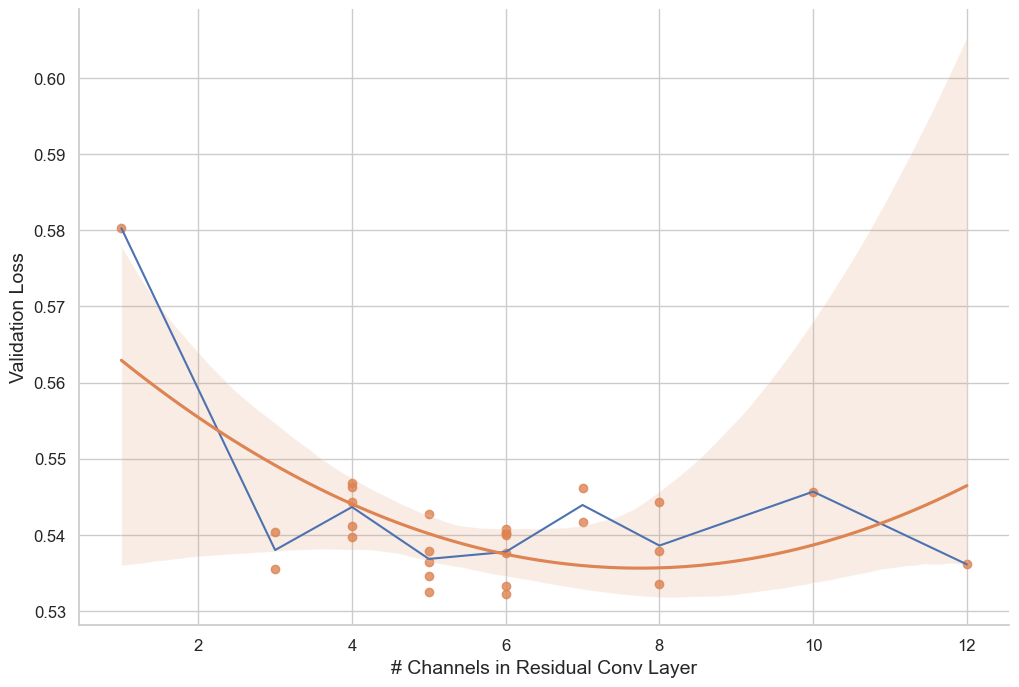
\includegraphics[width=0.45\textwidth]{figures/06_ModelExploration/4_CNN/conv_chskip.png}
    \caption{Influence of the number of channels in the skip connection.}
    \label{fig:ch_skip}
\end{figure}

Given the low number of optimization trials used to evaluate  \( C_{\text{out}}^{(\text{skip})} \), we decided to choose
a more conservative value of \( C_{\text{out}}^{(\text{skip})} = 5 \) to avoid overfitting. \\
Empirical evidence indicated a marginal performance increase when applying the \gls{relu} activation function to the
output of the skip connection. Its application post-concatenation introduces non-linearity that helps in the differentiation
and processing of features. Given its low
computational overhead and subtle positive impact on model performance, we decided to apply ReLU to our skip connections, thereby
leveraging the advantages of non-linearity while maintaining computational efficiency.

\paragraph{Varying Snapshot Count}
\hyperref[fig:cnn_plus_arch]{Figure~\ref*{fig:cnn_plus_arch}} conceptualizes the adaptation of the employed CNN architecture to handle a variable number
of snapshots by embedding the number of snapshots \( K \) into the skip branch of the network.
The results of the evaluation of the model with varying snapshot count will be presented in~\autoref{sec:influence_num_snapshots}.

\subsection{Resulting Architecture}
\label{subsubsec:resulting_architecture}

The development of the \gls{cnn} architecture, delineated in~\autoref{fig:cnn_architecture}, was achieved through a
methodical hyperparameter optimization facilitated by \textsc{Optuna}.
The optimization targeted a multidimensional objective function that accounted for validation loss (\( \meanLossCEVal \)),
model complexity (number of parameters and \glspl{mac}), and validation accuracy (\( \meanAccVal \)).

\begin{figure}[H]
    \centering
    \subfloat[]{{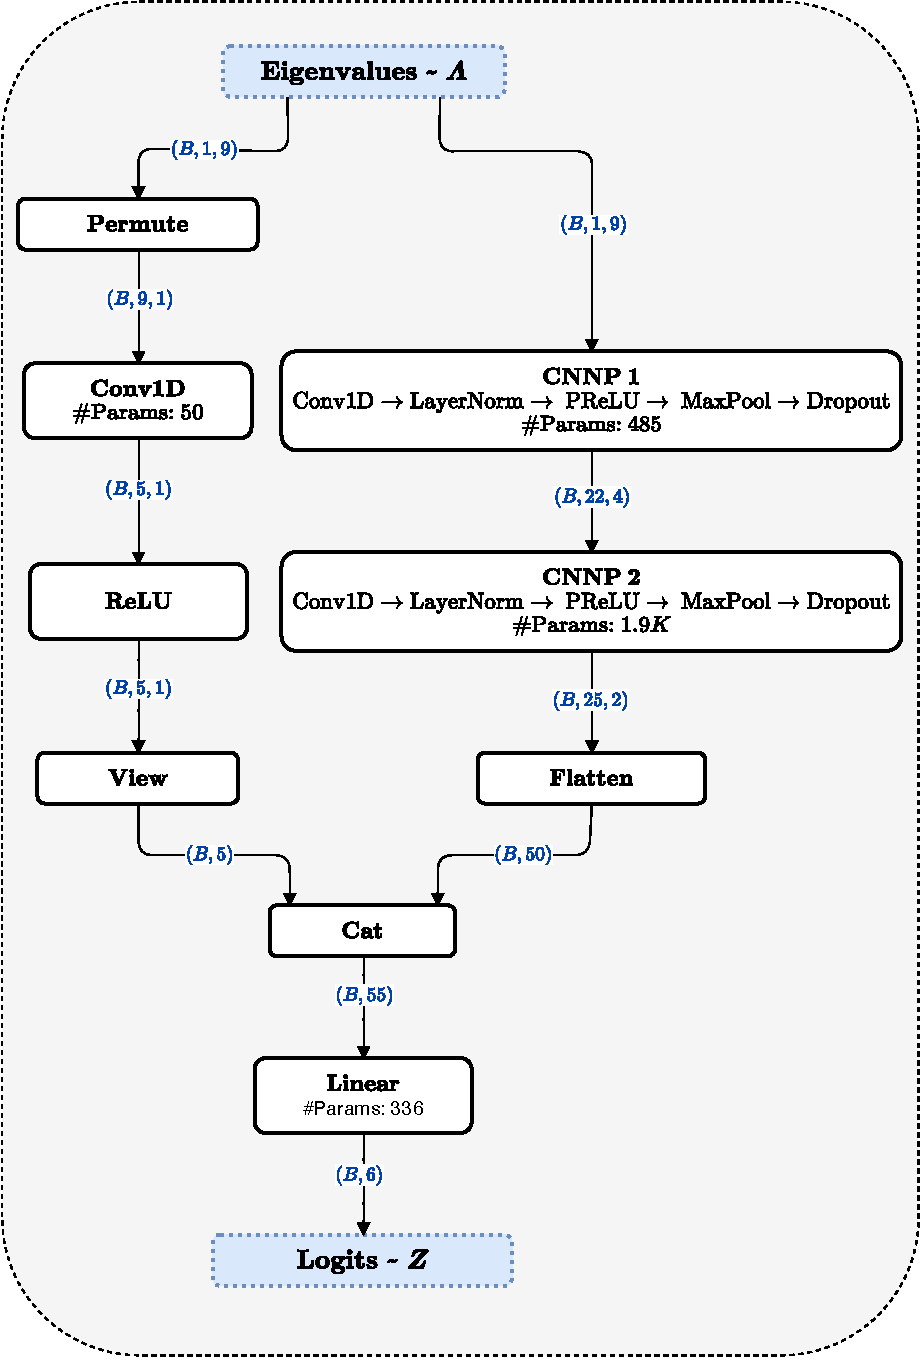
\includegraphics[width=0.41\textwidth]{figures/06_ModelExploration/4_CNN/cnn.pdf}}}
    \hspace{0.5cm}
    \subfloat[\label{fig:cnn_plus_arch}]{{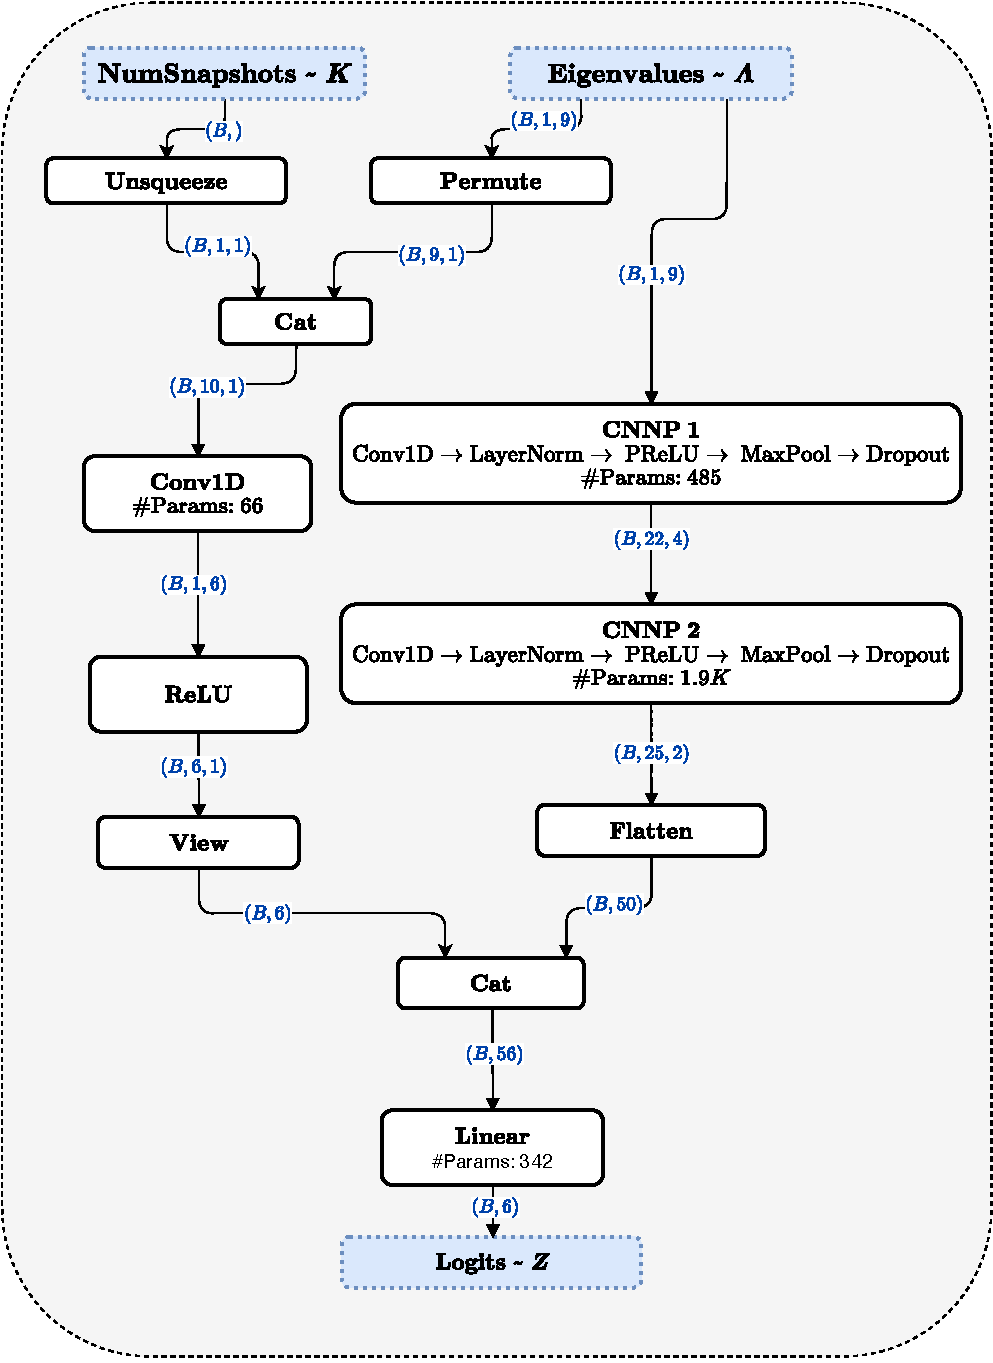
\includegraphics[width=0.44\textwidth]{figures/06_ModelExploration/4_CNN/cnn+.pdf}}}
    \caption{Schematic of the \gls{cnn} (a) and its variable snapshot adaptation (b).}
    \label{fig:cnn_architecture}
\end{figure}

The decision to employ a series connection of two \texttt{CNNP}'s in the ``main'' path can be attributed to the length
of the input sequence \( L_{\text{seq}} = M\), which is short enough, such that two \texttt{CNNP} blocks with kernel
sizes of three in combination with the adaptive max pooling%
\footnote{The dimensional reductions are denoted in~\autoref{tab:cnn_summary}}
layers can effectively capture relevant features at all spatial scales. \\
Experimental evaluations indicated that the addition of a third \texttt{CNNP} block without intermediate pooling did not
affect performance, while a singular \texttt{CNNP} block increased validation loss.

Detailed hyperparameters and layer configurations that underpin the network's structure and training methodology are
summarized in~\autoref{tab:cnn_summary}.

\begin{table}[H]
    \centering
    \caption{Summary of Hyperparameters and Layer Configurations}
    \label{tab:cnn_summary}
    \resizebox{\textwidth}{!}{%
    \begin{tabular}{@{}lll@{}}
    \textbf{Block / Module}               & \textbf{Child}        & \textbf{Parameters / Value}            \\ \midrule
    \multicolumn{3}{l}{\textbf{Modules}}                                                     \\ \midrule
    \multirow{7}{*}{\texttt{CNNP} Block 1}
                                         & \texttt{nn.Conv1d}           & Channels: \(1 \rightarrow 22\), Kernel Size: 3, Padding: \texttt{reflect} \\
                                         &                              & \#Params \( = C_{\text{in}} \times C_{\text{out}} \times k + C_{\text{out}} = 88\) \\
                                         & \texttt{nn.Layer Norm}        & \#Params \( = 2 \times C_{\text{out}} \times L_{\text{seq}} = 396 \) \\
                                         & \texttt{nn.PReLU}                & \#Params = 1            \\
                                         & \texttt{AdaptiveMaxPool1d}&  \(L_{\text{seq}} : 9 \rightarrow 4 \)                   \\
                                         & \texttt{nn.Dropout}          & Rate: 0.06                      \\
                                         & \( \Sigma \) \#Params                  &  \( 1 \times 22 \times 3 + 2 + 2 \times 22 \times 9 + 1 = 485 \)\\\midrule
    \multirow{7}{*}{\texttt{CNNP} Block 2}
                                         & \texttt{nn.Conv1d}           & Channels: \(22 \rightarrow 25\), Kernel Size: 3, Padding: \texttt{reflect} \\
                                         &                              & \#Params \( = C_{\text{in}} \times C_{\text{out}} \times k + C_{\text{out}} = 1675\) \\
                                         & \texttt{nn.Layer Norm}        & \#Params \( = 2 \times C_{\text{out}} \times L_{\text{seq}} = 200 \)                       \\
                                         & \texttt{nn.PReLU}                & \#Params = 1            \\
                                         & \texttt{nn.AdaptiveMaxPool1d}& \(L_{\text{seq}} : 4 \rightarrow 2 \)                   \\
                                         & \texttt{nn.Dropout}                   & Rate: 0.06                      \\
                                         & \( \Sigma \) \#Params                & \( 22 \times 25 \times 3 + 25 + 2 \times 25 \times 4 + 1 = 1876 \) \\\midrule
    \multirow{3}{*}{Skip Connection}     & \texttt{nn.Conv1d}          & Channels: \(9 \rightarrow 5\), Kernel Size: 1 \\
                                         &                              & \#Params \( = C_{\text{in}} \times C_{\text{out}} + C_{\text{out}} = 50 \) \\
                                         & \texttt{nn.ReLU}                &             \\ \midrule
    Head                                 & \texttt{nn.Linear}          & \#Params = \( (2 \times 25 + 5) \times \| \NSet \| + \| \NSet \| = 336 \) \\
    \midrule[0.1pt]
    \addlinespace[0.5cm]
    \( \Sigma \) \#Params                & \texttt{ConvNet8} & 2747 \\
    \bottomrule

    \addlinespace[1cm]
    \multicolumn{3}{l}{\textbf{Non-Layer Hyperparameters}}                                       \\ \midrule
    Optimizer                            &                           & \texttt{optim.AdamW} \\
    Batch Size                           &                           & 512                       \\
    Learning Rate                        &                           & 0.002                     \\
    Weight Decay                         &                           & 0.01685                   \\
    LR Scheduler                         &                           & \texttt{lr\_scheduler.ReduceLROnPlateau}\\
    Precision                            &                           & \texttt{32-true}     \\
    \bottomrule
    \end{tabular}%
    }
\end{table}

\autoref{tab:cnn_summary} presents the chosen hyperparameters, notably including the \texttt{AdamW} optimizer. \\
This optimizer modifies the \texttt{Adam} algorithm by applying weight decay directly to the model weights instead of
incorporating it into the gradient updates. This approach allows \texttt{AdamW} to achieve more effective regularization,
enhancing the model's generalization capabilities by decoupling weight decay from the learning rate's adaptive adjustments~\cite{loshchilov2019decoupled}.

While a batch size of 1024 was used during the optimization process, the final model was trained with a batch size of 512%
\footnote{A short optimization run yielded a batch size of \( \B = 504 \) as optimal value.},
as the latter yielded a lower validation loss. This can be attributed to the fact that lower batch sizes intorduce more noise
to the optimization process, which can be beneficial to escape sharp local minima, and thus improve the generalization capabilities.

Furthermore, we employed \texttt{ReduceLROnPlateau} as a learning rate scheduler.
A comparison with other suitable
learning rate schedulers, such as \texttt{CyclicLR}, \texttt{OneCycleLR}, and
\texttt{CosineAnnealingLR}, did not yield actionable insights, as the number of steps per epoch
was too high to effectively utilize any of these schedulers. \\
An effective way to overcome this issue will be introduced in~\autoref{subsub:training_data}.

The learning rate, weight decay and dropout rate have also been optimized. The results of this optimization process can
be found in the appendix -- see Figures~\ref{fig:dropout_cnn},~\ref{fig:lr_cnn}, and~\ref{fig:wd_cnn}. \\
The weight decay parameter was optimized solely for the \gls{cnn} and was uniformly applied to all yet to be introduced
models.

\newpage{}

\section{Multilayer Perceptron}
\label{sec:mlp}

Advancements in the field of deep learning over the past decade have underscored the superiority of convolutional
and recurrent neural networks over traditional feedforward architectures, such as the \glsfirst{mlp}.\\
This superiority largely stems from CNNs' and RNNs' inherent abilities to capture spatial and temporal dependencies within
data.
Additionally, both CNNs and RNNs employ parameter sharing mechanisms -- across space for CNNs, and across time for \glspl{rnn}
-- decreasing their susceptibility to overfitting.\\

Nonetheless, the \gls{mlp} remains a foundational architecture worth exploring. This is especially true for tasks of low
complexity, where the risk of overfitting is low and the data not inherently spatially or temporally dependent.\\
However, the \gls{mlp} architecture has not been explored as extensively as the \gls{cnn} and \gls{rnn} architectures, and
is mostly an analogue to the previously introduced \gls{cnn} architecture.\\
Hence, the deep feed forward architecture will be a composite of \texttt{MLPBlock}s, each consisting of a linear layer,
followed by a normalization layer, a non-linear activation function, and finally a dropout layer. \\

\subsection{Hyperparameter Optimization}


\subsubsection{Number of Features}
\begin{figure}[H]
    \centering
    \subfloat[\texttt{MLPBlock 1}]{{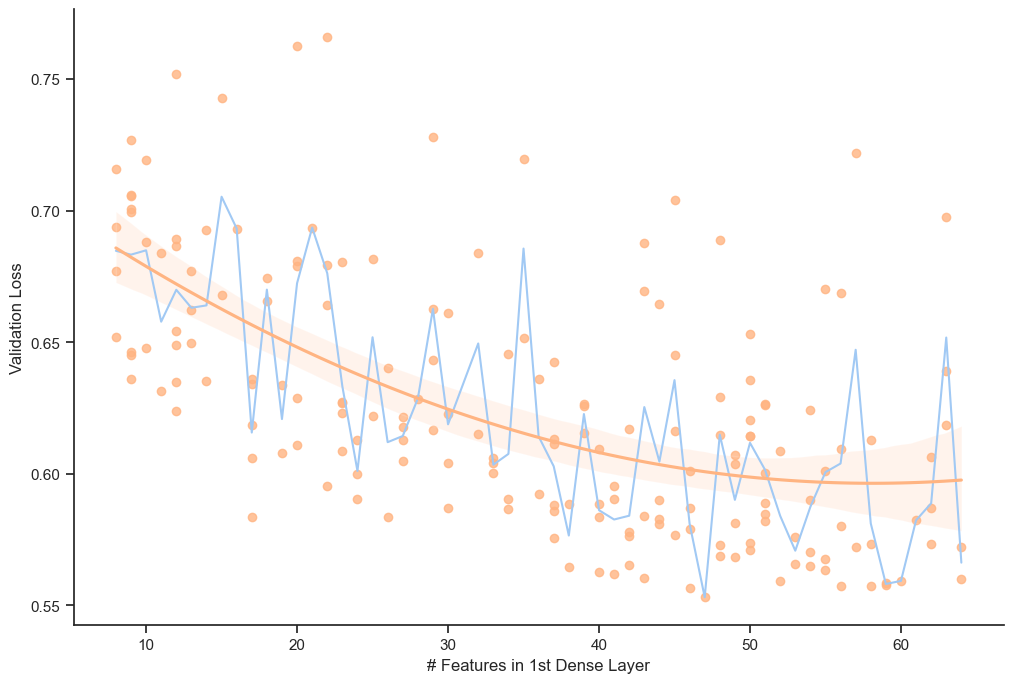
\includegraphics[width=0.33\textwidth]{figures/06_ModelExploration/5_MLP/ch1.png
    }}}
    \subfloat[\texttt{MLPBlock 2}]{{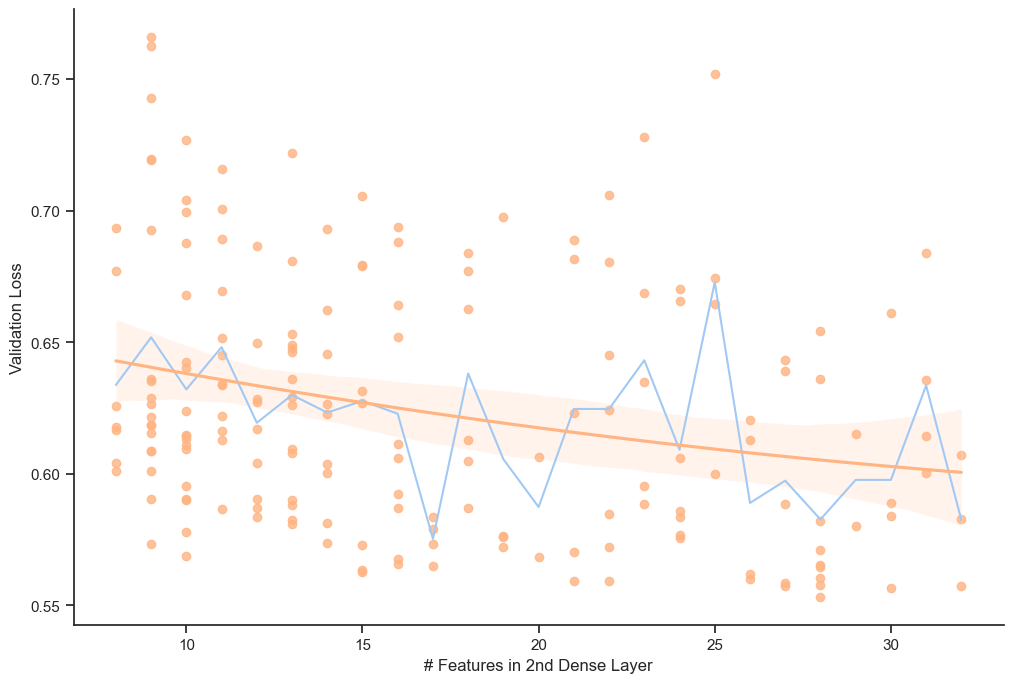
\includegraphics[width=0.33\textwidth]{figures/06_ModelExploration/5_MLP/ch2.png
    }}}
    \subfloat[\texttt{MLPBlock 3}]{{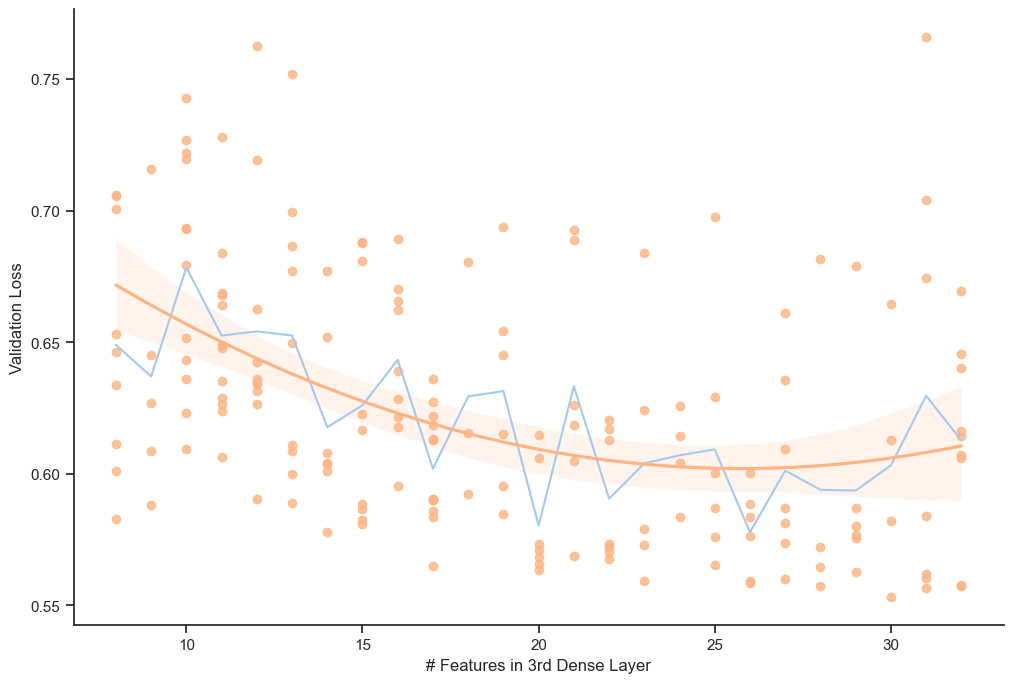
\includegraphics[width=0.33\textwidth]{figures/06_ModelExploration/5_MLP/ch3.png
    }}}
    \caption{Regression plots of the \( \lossCEVal \) for different numbers of features in the three \texttt{MLPBlock}s.}
    \label{fig:mlp_features}
\end{figure}

The exploration of the optimal number of features in the \texttt{MLPBlock}s, as depicted in \autoref{fig:mlp_features},
revealed a monotonically decreasing trend in validation loss with an increase in feature numbers for the second block, while
the first and third blocks each exhibited a local optimum within the explored range. \\
This observation suggests a higher feature count could potentially enhance model performance.
However, considering the stronger relative influence of the number of features in the first and third layers, the
feature count for the second \texttt{MLPBlock} was set to a rather conservative value of 20, to mitigate model complexity and
potential overfitting.

In retrospect, this decision seems doubious, as the subsequent \texttt{MLPBlock} contains four more features than block
two. This might cause an unwanted bottleneck effect and make some information in the last block redundant.\\


\subsubsection{Normalization and Residual Connection}

\begin{table}[H]
    \centering
    \caption{Comparison of MLP Variants}
    \label{tab:mlp_variants}
    \begin{tabular}{@{}lccccc@{}}
    \toprule
    Configuration & \multicolumn{2}{c}{\( \meanLossCEVal \)} & \multicolumn{2}{c}{\( \meanAccVal \)} \\
    \cmidrule(lr){2-3} \cmidrule(lr){4-5}
                  & \( \nu \) & \( \%\Delta \) & \( \nu \) & \( \%\Delta \) \\
    \midrule
    \multicolumn{5}{l}{Normalization} \\
    False          & 0.657 & - & 0.696 & - \\
    Batch Norm     & 0.656 & \gnbx{-0.208} & 0.706 & \gnbx{1.429} \\
    Instance Norm  & 0.621 & \gnbx{-5.567} & 0.717 & \gnbx{3.011} \\
    Layer Norm     & 0.596 & \gnbx{-9.245} & 0.728 & \gnbx{4.594} \\
    \midrule
    \multicolumn{5}{l}{Skip Connection} \\
    False          & 0.657 & - & 0.695 & - \\
    Skip           & 0.611 & \gnbx{-7.078} & 0.723 & \gnbx{4.067} \\
    \bottomrule
    \end{tabular}
\end{table}


The examination of normalization methods and skip connections within the MLP architecture reveals that both modifications
significantly influence model performance.\\
Normalization, particularly Layer Norm, markedly enhances model accuracy and reduces validation loss,
highlighting its role in stabilizing the training process and improving generalization.
Since the \gls{mlp}'s internal tensors do not exhibit separate spacial or temporal dimensions together with a channel
dimension, Instance Norm and Batch Norm aggregate their statistics in the same manner. Their difference lies in the
subsequent scaling and shifting operations.\\
While Layer Norm uses individual scaling and shifting parameters (\( \bfm{\gamma}, \bfm{\beta} \)) for each feature,
it was not possible to instantiate Instance Norm with the inclusion of the subsequent affine transformation.

The integration of skip connections also shows a notable positive effect on the model's performance.
The linear transformation within the skip branch, designed to align the feature count with the final \texttt{MLPBlock}, is then
added to the last \texttt{MLPBlock}'s output.
This addition introduces only a marginal increase in model complexity, with \( 9 \times ( 24 + 1) = 225 \) additional parameters.\\


\subsection{Resulting Architecture}
\label{sub:mlp_architecture}

The \gls{mlp} model used for testing and final comparative analysis is visualized in \autoref{fig:mlp_model}.\\
Unfortunately, the skip connection, which is highlighted in purple in the diagram, was not implemented into the final model as initially intended.

\begin{figure}[H]
    \centering
    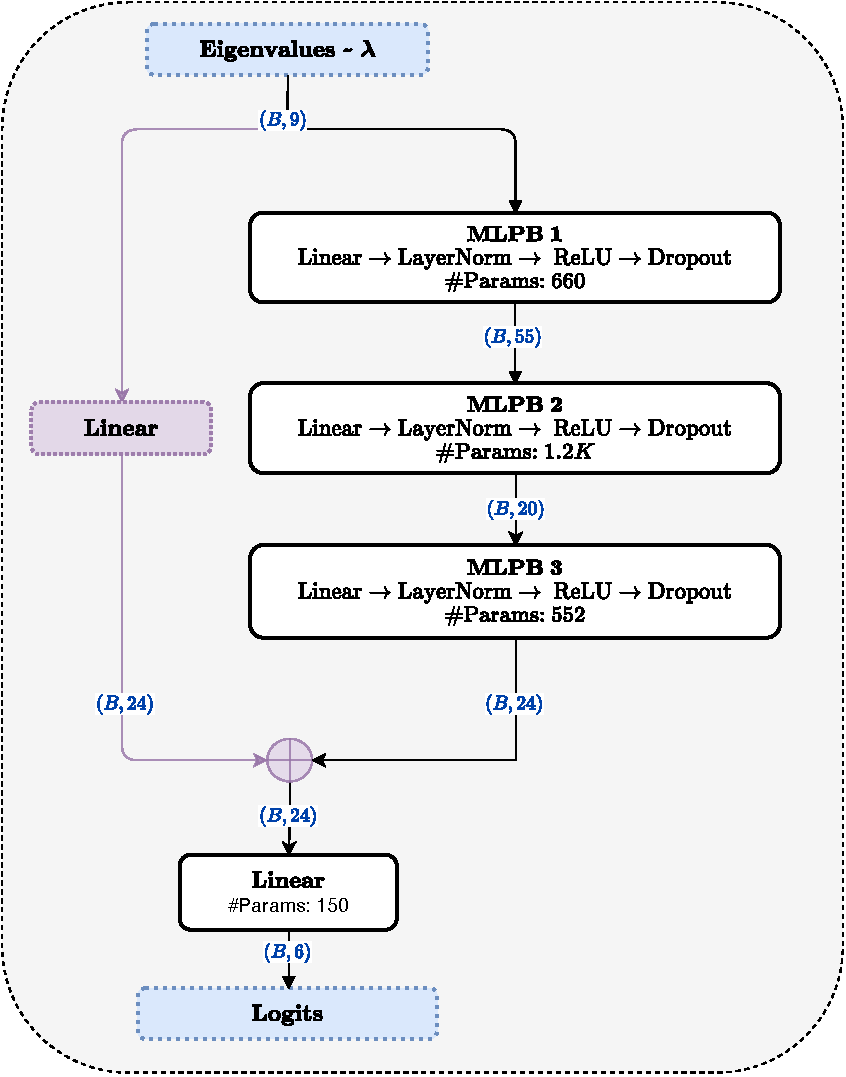
\includegraphics[width=0.45\textwidth]{figures/06_ModelExploration/mlp.pdf}
    \caption{Flowchart of the MLP architecture.}
    \label{fig:mlp_model}
\end{figure}

The architecture, as depicted, encapsulates a sequential arrangement of three \texttt{MLPBlock}s, each comprising essential
components for a feedforward network: linear transformation, normalization, activation, and regularization through
dropout.\\

\autoref{tab:mlp_summary} summarizes the hyperparameters and layer configurations of the final \gls{mlp} model.

\begin{table}
    \centering
    \caption{Summary of Hyperparameters and Layer Configurations for DenseNet}
    \label{tab:mlp_summary}
    \small
    \begin{tabular}{@{}lll@{}}
    \toprule
    \textbf{Block / Module}               & \textbf{Child}        & \textbf{Parameters / Value}            \\ \midrule
    \multicolumn{3}{l}{\textbf{Modules}}                                                     \\ \midrule
    \multirow{7}{*}{\texttt{MLPBlock} 1} & \texttt{nn.Linear}           & Features: \(9 \rightarrow 55\) \\
                                         &                              & \#Params \( = 9 \times 55 + 55 = 550\) \\
                                         & \texttt{nn.LayerNorm}        & \#Params \( = 2 \times 55 = 110\) \\
                                         & \texttt{nn.ReLU}             & \\
                                         & \texttt{nn.Dropout}          & Rate: 0.06                      \\
                                         & \( \Sigma \) \#Params        & 660 \\ \midrule
    \multirow{6}{*}{\texttt{MLPBlock} 2} & \texttt{nn.Linear}           & Features: \(55 \rightarrow 20\) \\
                                         &                              & \#Params \( = 55 \times 20 + 20 = 1120\) \\
                                         & \texttt{nn.LayerNorm}        & \#Params \( = 2 \times 20 = 40\) \\
                                         & \texttt{nn.ReLU}             & \\
                                         & \texttt{nn.Dropout}          & Rate: 0.06                      \\
                                         & \( \Sigma \) \#Params        & 1160 \\ \midrule
    \multirow{6}{*}{\texttt{MLPBlock} 3} & \texttt{nn.Linear}           & Features: \(20 \rightarrow 24\) \\
                                         &                              & \#Params \( = 20 \times 24 + 24 = 504\) \\
                                         & \texttt{nn.LayerNorm}        & \#Params \( = 2 \times 24 = 48\) \\
                                         & \texttt{nn.ReLU}             & \\
                                         & \texttt{nn.Dropout}          & Rate: 0.06                      \\
                                         & \( \Sigma \) \#Params               & 552 \\ \midrule
    Head                                 & \texttt{nn.Linear}           & \#Params \( = 24 \times \| \NSet \| + \| \NSet \| = 150\) \\
                                         &                              & \#Params = 150 \\
    \midrule[0.1pt]
    \addlinespace[0.5cm]
    \( \Sigma \) \#Params                & \texttt{DenseNet} & 2522 \\
    \bottomrule

    \addlinespace[1cm]
    \multicolumn{3}{l}{\textbf{Non-Layer Hyperparameters}}                                       \\ \midrule
    Optimizer                            &                           & \texttt{optim.AdamW} \\
    Batch Size                           &                           & 512                       \\
    Learning Rate                        &                           & 0.005                     \\
    Weight Decay                         &                           & 0.01685                   \\
    LR Scheduler                         &                           & \texttt{lr\_scheduler.ReduceLROnPlateau}\\
    Precision                            &                           & \texttt{32bit-true}     \\
    \bottomrule
    \end{tabular}
\end{table}

Without any further hyperparameter optimization, the learning rate of the final model was set to a value of
\( \alpha = 0.005 \)%
\footnote{Retrospectively, this value seems to be too high, as argumented in~\autoref{subsub:considerations_nn}.}.
The weight decay, as well as the dropout rate have been adapted from the convolutional model.\\

\subsubsection{Future Improvements}

Given the freedom of choice with respect to the number of features in the \texttt{MLPBlock}s, an adaptation worth considering
would be to align the feature count in the second \texttt{MLPBlock} to match the third could mitigate potential information
bottlenecking and enable the model to leverage a broader feature representation. This adjustment might not only harmonize
the flow of information across the layers but could also pave the way for implementing a true residual connection,
paralleling the final \texttt{MLPBlock}, to further enhance the model's learning capacity without substantially increasing its complexity.

Should the model be considered for further development, it would also be interesting to explore the impact of pruning
techniques on the model's performance.\\

The observed slight performance improvements through the use of \gls{prelu} over \gls{relu} in the convolutional model
suggest that these findings could be transferred to the \gls{mlp} model.\\

Moreover, considering the future development of the model, the application of pruning techniques could be investigated
to refine the network's architecture by identifying and eliminating redundant units or connections, thereby streamlining
the model for improved efficiency.

\section{Recurrent Neural Network}

\subsection{Hyperparameter Optimization}

This section explores the architecture of \glspl{rnn} tailored for our task. RNNs excel in processing sequential data,
making them an intuitive architectural choice under the assumption that the ordered eigenvalues should contain ``temporal'' information.\\
The section aims to investigate various architectural choices, including cell type, sequence order, and bidirectionality, to identify the
most effective configuration for the task at hand. \\
The iterative application of the same weights across sequence elements aligns well with the potential goal of using the
model in an \gls{fpga} implementation, where weight sharing can lead to significant efficiency gains.\\

Since a detailed theoretical introduction to \glspl{rnn} would be helpful for the following consideration of the effects of
certain RNN specific architecture decisions, but would
exceed the scope of this work, we refer to the literature~\cite[Chapter 10.2 ff.]{dlbook} for a comprehensive introduction to
\glspl{rnn} or to~\cite{dlcheatsheet} for a more compact overview.\\

\subsubsection{Selection of the RNN Cell Type}

Among the various \gls{rnn} cell types, the classic \gls{rnn} cell was chosen over \gls{lstm} and \gls{gru} cells. This
decsision will be substantiated through the combination of empirical findings and theoretical considerations, which will
be presented in this section.\\

\begin{figure}[H]
    \centering
    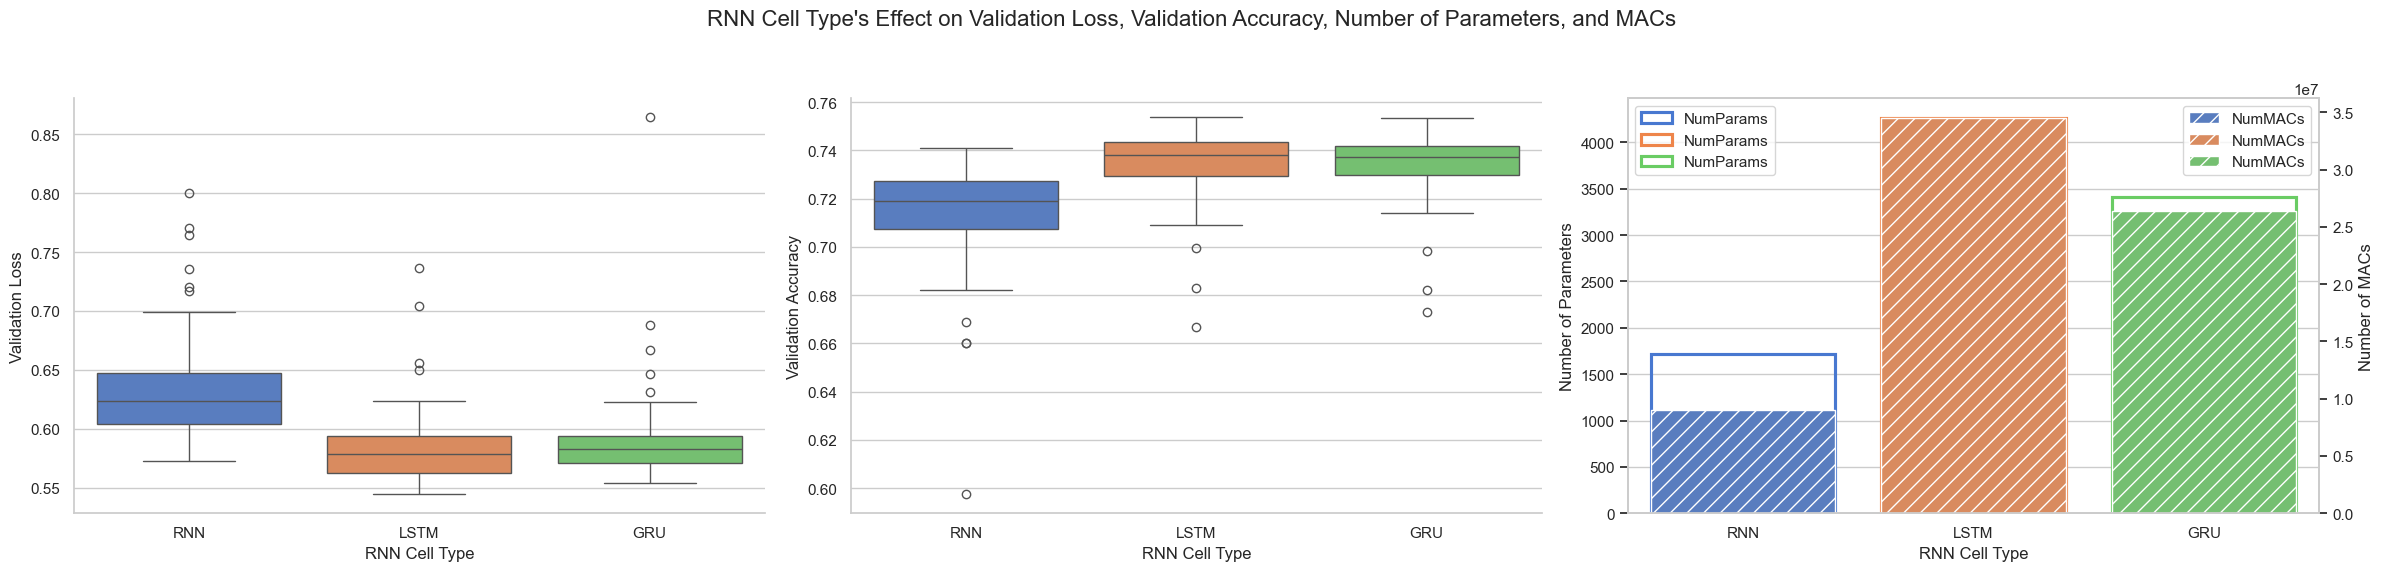
\includegraphics[width=1\textwidth]{figures/06_ModelExploration/RNN/rnn_cell_types.png}
    \caption{Comparison of RNN cell types with respect to validation loss, validation accuracy, and computational complexity.}
    \label{fig:rnn_cell_types}
\end{figure}

\begin{table}[H]
    \centering
    \caption{Comparison of Different RNN Cell Types}
    \label{tab:rnn_cell_types}
    \begin{tabular}{@{}lcccccccc@{}}
    \toprule
    & \multicolumn{2}{c}{\( \meanLossCEVal \) } & \multicolumn{2}{c}{ \( \meanAccVal \) } & \multicolumn{2}{c}{\#Params} & \multicolumn{2}{c}{\#MACs} \\
    \cmidrule(lr){2-3} \cmidrule(lr){4-5} \cmidrule(lr){6-7} \cmidrule(lr){8-9}
    RNN Cell Type & \( \nu \) & \( \%\Delta \) & \( \nu \) & \( \%\Delta \) & \( \nu \) & \( \%\Delta \) & \( \nu \) & \( \%\Delta \) \\
    \midrule
    RNN  & 0.634 & —             & 0.714 & —            & 1718 & —          & 8784  & —           \\
    GRU  & 0.591 & \gnbx{-6.72}  & 0.734 & \gnbx{2.76} & 3414 & \rdbx{98.7} & 25780 & \rdbx{193}\\
    LSTM & 0.585 & \gnbx{-7.78}  & 0.734 & \gnbx{2.84} & 4262 & \rdbx{148}  & 33700 & \rdbx{283}\\
    \bottomrule
    \end{tabular}
\end{table}

This choice is substantiated by the empirical findings presented in~\autoref{tab:rnn_cell_types} and~\autoref{fig:rnn_cell_types},
which compare the cell types based on performance and computational demands, revealing the traditional RNN cell as the most balanced option.\\
The significantly lower computational complexity of the RNN cell, compared to GRU and LSTM cells, stems from its simpler
structure without gating mechanisms. Each gate in GRU and LSTM cells—two for GRU and three for LSTM—requires its own
set of parameters and non-linear operations, specifically \( \operatorname{sigmoid} \) and \( \operatorname{tanh} \) functions.
In contrast, the traditional RNN relies on a single \( \operatorname{tanh} \) activation function, markedly reducing the
number of parameters and computational operations required.

The purpose of the gating mechanisms in GRU and LSTM cells is to manage the temporal flow of information, allowing the model to
retain or discard information as needed. This capability is particularly beneficial for long sequences with high complexity, where the
incorporation of dependencies over extended temporal horizons with varying correlations is an intricate task. Furthermore, the
vanishing gradient problem is more likely to compromise the model's ability to capture long-term dependencies.\\
However, the relatively short sequence length, determined by the number of antennas \( M \), and low complexity of our input data,
alleviate concerns related to the vanishing gradient problem or dependencies with temporal dispersion, making the traditional
RNN cell a suitable choice for the given tasks.\\

\subsubsection{Further Architectural Considerations}

The exploration of the hyperparameter space for the RNN architecture extends beyond the selection of the cell type.\\
Further architectural considerations include the sequence order, bidirectionality, and the integration of convolutional
layers for enhanced feature extraction.\\
Additionally, a fine-tuning of hyperparameters, such as the number of hidden units and learning rate was conducted. \\


\begin{figure}[H]
    \centering
    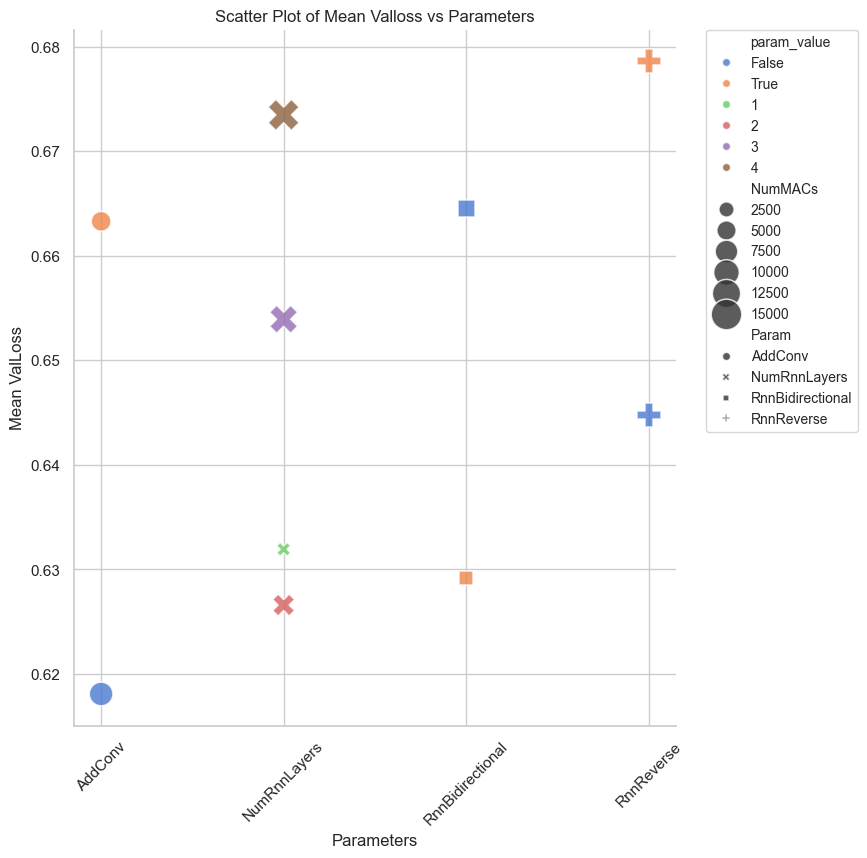
\includegraphics[width=0.6\textwidth]{figures/06_ModelExploration/RNN/rnn_scatter.png}
    \caption{Comparison of various hyperparameters with respect to the mean validation loss.}
    \label{fig:rnn_scatter}
\end{figure}

\autoref{fig:rnn_scatter} illustrates the impact of different hyperparameters on the mean validation loss \( \meanLossCEVal \) and
also aims to deliver a rather qualitative dependence of the model complexity in terms of \glspl{mac} by the marker sizes.\\
The impacts of theses architectural considerations depicted in~\autoref{fig:rnn_scatter} are furthermore gathered in~\autoref{tab:model_variants}:

\begin{table}[H]
    \centering
    \caption{Comparison of Model Variants}
    \label{tab:model_variants}
    \begin{tabular}{@{}lcccccccc@{}}
    \toprule
    & \multicolumn{2}{c}{\( \meanLossCEVal \) } & \multicolumn{2}{c}{ \( \meanAccVal \) } & \multicolumn{2}{c}{\#Params} & \multicolumn{2}{c}{\#MACs} \\
    \cmidrule(lr){2-3} \cmidrule(lr){4-5} \cmidrule(lr){6-7} \cmidrule(lr){8-9}
    Configuration & \( \nu \) & \( \%\Delta \) & \( \nu \) & \( \%\Delta \) & \( \nu \) & \( \%\Delta \) & \( \nu \) & \( \%\Delta \) \\
    \midrule[0.2pt]
    One Layer  & 0.632 &   —            &  0.717&   —            & 638  &   —           &  1830 &   —  \\
    Two Layers & 0.627 &   \gnbx{-0.844}&  0.718&   \gnbx{0.192}&  1470 &   \rdbx{130}&  6948 &   \rdbx{280}   \\
    \midrule[0.2pt]
    Without \texttt{CNNP} & 0.618 & —             & 0.724 & —             & 1287 & —       & 5308        &     — \\
    With \texttt{CNNP}    & 0.663 & \rdbx{7.31}    & 0.701  & \rdbx{-3.19}   & 1503 & \rdbx{17.6} & 8304 & \rdbx{56.4} \\
    \midrule[0.2pt]
    Unidirectional  & 0.665 & —             & 0.701 & —             & 1256 & —       & 5728 & — \\
    Bidirectional   & 0.629 & \gnbx{-5.32}   & 0.718 & \gnbx{2.34}    & 1648 & \rdbx{31.2} & 8707 & \rdbx{52.0} \\
    \midrule[0.2pt]
    Descending Order & 0.645 & —             & 0.710   & —             & 1701 & —       & 8825 & — \\
    Ascending Order  & 0.679 & \rdbx{5.24}    & 0.695 & \rdbx{-2.07}   & 1610 & — & 8624 & — \\
    \bottomrule
    \end{tabular}
\end{table}

\paragraph{Vertical Depth}
The vertical depth of an RNN refers to the number of recurrent cells stacked on top of each other to form a
deeper network architecture. Each non-final layer's output constitutes the input to the subsequent layer.\\
This concept should become clear through the consideration of~\autoref{fig:rnn_architecture}, which depicts the unrolled
architecture of the fineal RNN model. The RNN cell \( \mathrm{RNN}^{\rightarrow}_{t, 1} \) is the first layer of the RNNs
forward path, and its output is subsequently fed into the second RNN cell \( \mathrm{RNN}^{\rightarrow}_{t, 2} \). \\
Both cells exhibit their own set of weights, biases and hidden states.\\
The addition of a second RNN layer yields a marginal improvement, whereas the inclusion of further
layers causes the model to overfit on the training data. Although, the additional computational complexity introduced by
the additional layer can \emph{not} be justified by the marginal performance gain, it was unfortunately decided to utilize a
two-layered RNN architecture in the final model. \\
This decision can be attributed to an incorrect initial assessment of this hyperparameters impact on the model's performance.\\


\paragraph{Hybrid Architecture} The integration of a \texttt{CNNP} block from~\autoref{sec:cnn} was considered as an
initial feature extraction step. \\
The \texttt{CNNP}'s output \( \bfm{X} \in \mathbb{R}^{\B \times C_{\text{out}} \times 3} \) was permuted accordingly to~\autoref{eq:transposition_rnn}
and subsequently fed into the RNN. \\
However, empirical results indicated a performance detriment rather than a benefit, suggesting that direct processing of
the sequence by the RNN is more suitable.

\paragraph{Bidirectional Configuration}
The bidirectional RNN outperforms the unidirectional RNN in terms of validation loss and accuracy. \\
In a bidirectional RNN, the input sequence is processed by two separate RNN layers simultaneously—one moving
forward from the start to the end of the sequence and the other moving backward from the end to the start~\cite[Chapter 10.3]{dlbook}.
The outputs from these two layers at each time-step, capturing the respective past and future contextual information,
are combined by concatenation to form a single output that represents the full contextual understanding at
that point in the sequence.
This consolidated output is then utilized by subsequent layers in the network -- in our case, the fully connected classification head.


\paragraph{Sequence Order}
The model's performance is influenced by the order in which eigenvalues are presented in the input tensor.
Using \( \bfLT^{(\text{RNN})}_{:,::-1,:} \) to present eigenvalues in ascending order, akin to the approach of the \gls{eft} algorithm,
results in poorer performance. \\
This observation can be rationalized by considering that the most critical attributes are encapsulated within the signal
eigenvalues \( \bfL_{S} \) and their comparative magnitude relative to the smaller eigenvalues associated with noise.
By arranging the eigenvalues in descending order for input into the model, it ensures that these pivotal features are
introduced to the model at the outset. This arrangement guarantees that the RNN layers subject these significant features
to a more thorough processing over time, enhancing the model's ability to focus on and leverage these key elements for
improved performance.


\paragraph{Number of Hidden Units}
\begin{figure}[H]
    \centering
    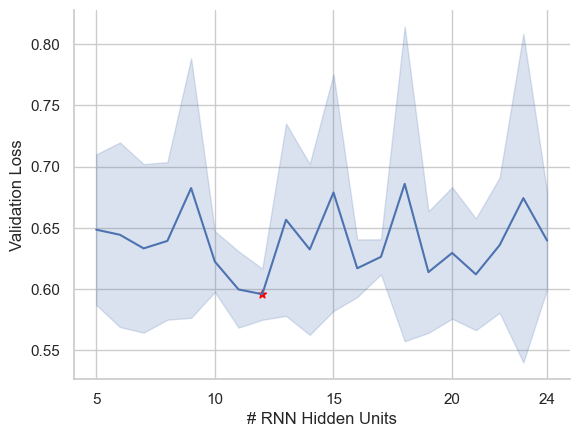
\includegraphics[width=0.5\textwidth]{figures/06_ModelExploration/RNN/rnn_num_hidden.png}
    \caption{Evaluation of the number of hidden units with respect to the mean validation loss.}
    \label{fig:rnn_hidden_units}
\end{figure}

The number of hidden units, denoted as \(H\), defines the dimensionality of the hidden state vector \(\bfm{h}_t\) at
each time step \(t\).\\
The impact of varying the number of hidden units on the mean validation loss, \(\meanLossCEVal\),
is illustrated in~\autoref{fig:rnn_hidden_units}.
A clear correlation between the number of hidden units and the mean validation loss is not evident. This observation led
to the selection of a conservative twelve hidden units -- \( \meanLossCEVal \) happens to exhibit a local minimum at this point.

The computation of the hidden state \(\bfm{h}_t\) at time step \(t\) is articulated by the following equation, which
integrates the influence of both the previous hidden state \(\bfm{h}_{t-1}\) and the current input \(\bfL_t\)~\cite{dlcheatsheet}:

\begin{equation}
    \bfm{h}_t = \operatorname{g}(\bfm{W}_{hh} \bfm{h}_{t-1} + \bfm{W}_{h\lambda} \bfL_t + \bfm{b}_h), \quad \operatorname{g} \in \{\operatorname{tanh}, \operatorname{ReLU}\}
    \label{eq:rnn_hidden_state}
\end{equation}

Here, \(\bfm{W}_{hh} \in \mathbb{R}^{H \times H}\) and \(\bfm{W}_{h\lambda} \in \mathbb{R}^{H \times M}\),
are the weight matrices, \( M \) is the dimensionality of the input vector containing the eigenvalues \( \bfL \), and
\(H\) is the number of hidden units.

\paragraph{Activation Function} The selection of non-linearities (\( g \)) for RNN cells in \textsc{PyTorch} is confined to
the \(\operatorname{tanh}\) and \(\operatorname{ReLU}\) functions. \\
The \(\operatorname{tanh}\) function has been chosen as the activation function for RNN cells, as it is the default option
for \emph{deep} RNN architectures since it tends to produce fewer dead neurons compared to the \(\operatorname{ReLU}\) function in \emph{deep} networks~\cite{lecun1998}. \\
While \(\operatorname{tanh}\) mitigates the risk of exploding gradients, \(\operatorname{ReLU}\) diminishes the likelihood of
vanishing gradients~\cite{pascanu2013difficulty}.\\
Given the shallowness of the RNN architecture, \(\operatorname{ReLU}\) might present a viable alternative to \(\operatorname{tanh}\),
and would be worth further investigation in future work.

\subsection{Resulting Architecture}

\begin{figure}[H]
    \centering
    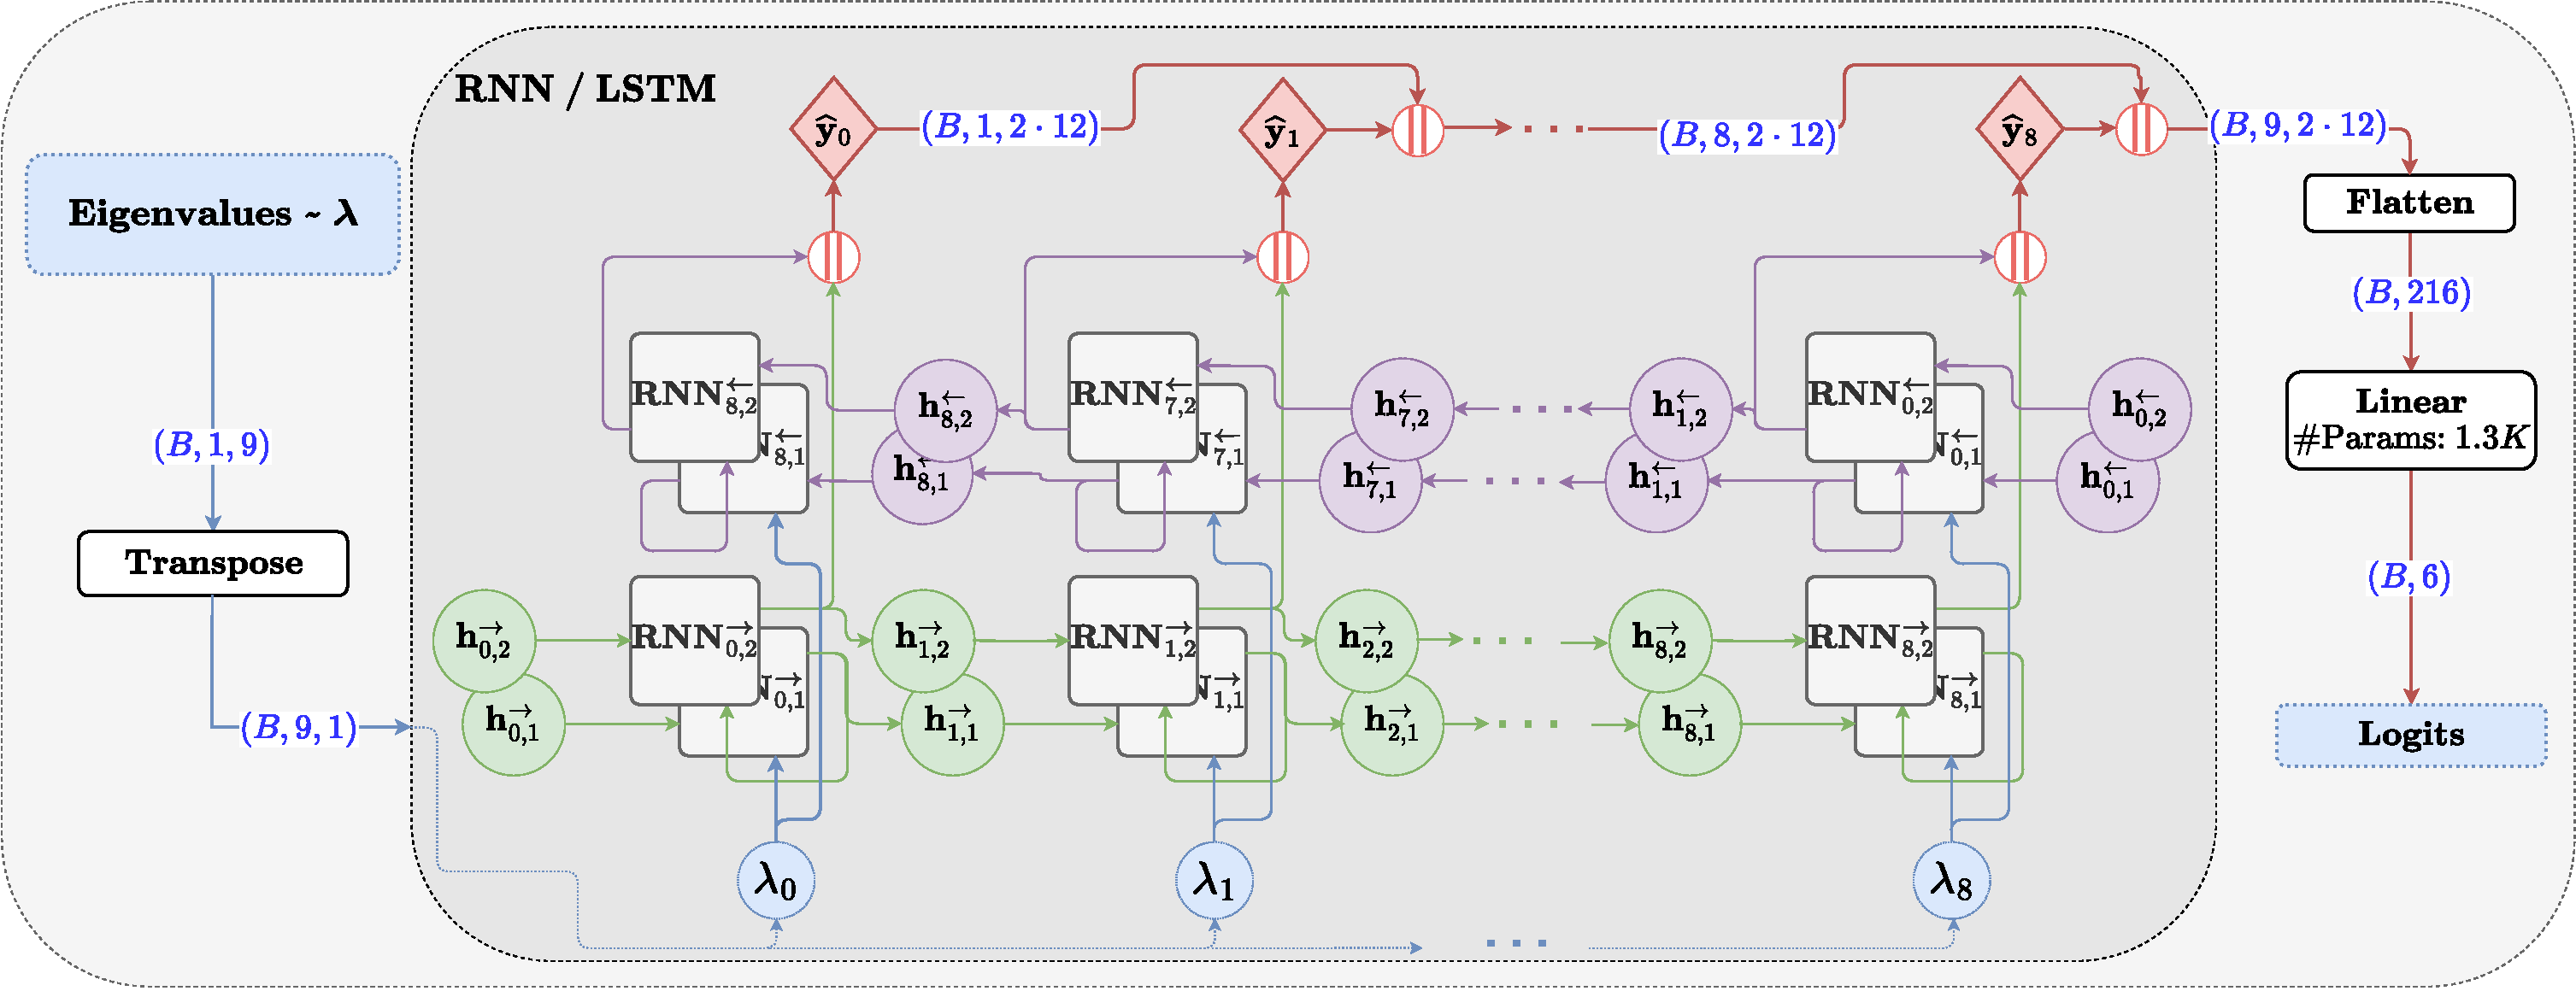
\includegraphics[width=1\textwidth]{figures/06_ModelExploration/RNN/rnn.pdf}
    \caption{Architecture of the unrolled bidirectional deep RNN.}
    \label{fig:rnn_architecture}
\end{figure}

The finalized architecture, as depicted in \autoref{fig:rnn_architecture}, embodies a deep, bidirectional RNN. \\
It leverages the capacity of bidirectional processing to capture the temporal dependencies from both forward \( \bullet^{\rightarrow} \)
and backward directions \( \bullet^{\leftarrow} \) of the input sequence.  \\
The deep structure, with two RNN layers (\( \mathrm{RNN}_{t,1} \rightarrow \mathrm{RNN}_{t,2} \)), enhances the model's
ability to abstract higher-level features, while maintaining computational efficiency.

This architecture is ``unrolled'' in the sense that it showcases each time step in the processing sequence, elucidating
the flow of data through the RNN cells. The input sequence is transposed to align the data for the bidirectional layers.\\
The RNN's output tensor has a shape of
\[
    (\B, L, D \cdot H), \quad \text{where}\: L = M, \: H = 12, \: D = \begin{cases}
                                                                    2 & \text{if bidirectional} \\
                                                                    1 & \text{otherwise.}
                                                                \end{cases}
\]
The output tensor is subsequently flattened and fed into a fully connected layer for the final classification. \\

The final model's hyperparameters and layer configurations are summarized in~\autoref{tab:rnn_summary}.
\begin{table}[H]
    \centering
    \caption{Summary of Hyperparameters and Layer Configurations for RNN Model}
    \label{tab:rnn_summary}
    \small
    \begin{tabular}{@{}lll@{}}
    \textbf{Block / Module}               & \textbf{Child}        & \textbf{Parameters / Value}            \\ \midrule
    \multicolumn{3}{l}{\textbf{Modules}}                                                     \\ \midrule
    \multirow{7}{*}{RNN Cell}
    & \texttt{nn.RNN} & Input Size: 1, Hidden Units: 12 \\
    & & Layers: 2, Bidirectional: \texttt{True}, Dropout: 0.06 \\
    & & Non-Linearity: \texttt{tanh}, \#Params: 1.3K \\
    & & \\
    & \texttt{nn.LSTM} & Input Size: 1, Hidden Units: 12 \\
    & & Layers: 2, Bidirectional: \texttt{True}, Dropout: 0.06 \\
    & & \#Params: 5.1K \\
    \midrule
    \multirow{2}{*}{Head}
    & \texttt{nn.Flatten}          &             \\
    & \texttt{nn.Linear}          & Features: \( 216 \rightarrow 6\), \#Params: 1302 \\
    \midrule[0.1pt]
    \addlinespace[0.5cm]
    \( \Sigma \) \#\(\text{Params}_{\text{RNN}}  \)               & & 2.6k\\
    \( \Sigma \) \#\(\text{Params}_{\text{LSTM}}  \)               & & 6.4k\\
    \bottomrule

    \addlinespace[1cm]
    \multicolumn{3}{l}{\textbf{Non-Layer Hyperparameters}}                                       \\ \midrule
    Optimizer                            &                           & \texttt{optim.AdamW} \\
    Batch Size                           &                           & 512                       \\
    Learning Rate                        &                           & 0.005                     \\
    Weight Decay                         &                           & 0.01685                   \\
    LR Scheduler                         &                           & \texttt{lr\_scheduler.ReduceLROnPlateau}\\
    Precision                            &                           & \texttt{32-true}     \\
    \bottomrule
    \end{tabular}%
\end{table}
The learning rate was chosen based on the results of an optimization study, as depicted in~\autoref{fig:rnn_lerning_rate}.
The dropout rate and weight decay were carried over from the \gls{cnn} architectures, and should be optimized for the RNN if
the model is to be further refined.\\

\subsubsection{Future Improvements}
\label{subsub:future_improvements_rnn}

While the current implementation utilizes all hidden states for the
final output, future versions could explore using only the last hidden state or selective slices of the sequence to
reduce the complexity of the dense layer.\\
Some units in the RNN's output layer might not carry relevant information. Especially the first units belonging to the
backward RNN might carry less relevant information that could be discarded.\\
This could be done by utilizing a pruning technique based on the resulting weights in the final layer.

Application of normalization techniques, such as layer normalization, could be beneficial to the RNN's performance, but
require a departure from the standard \texttt{nn.RNN} module to a custom implementation.\\

Without being able to provide a comprehensive analysis of the exploding or vanishing gradient problem, it is likely that
the occurrence of this issue is rather unlikely given the limited sequence length. Hence, the application of \texttt{ReLU}
as the activation function might be a viable alternative to \texttt{tanh} in future work.\\

The deployment of a deep \gls{rnn} architecture with two layers has shown a marginal improvement in performance metrics.
However, this negligible performance gain cannot be justified by the additional computational complexity.\\
Hence, it would be worthwhile to investigate the performance of a shallow \gls{rnn} architecture without having to anticipate
a significant performance loss.\\
Alternatively, the employment of a shallow \gls{gru} or \gls{lstm} architecture with an optimized number of hidden
units would be a more resource-conscious approach.\\


% END OF CHAPTER 6